\chapter{Re-organizing Vector Spaces into Interpretable Representations}\label{ch3}


\section{Introduction}\label{chapter3:Introduction}
%Representing the knowledge present in natural language data is a key task in Natural Language Processing. 




%One paragraph on why the lack of interpretability of document embeddings is an issue (i.e. what are the sorts of things we would like to do with document vectors that we can't do "off-the-shelf" with e.g. doc2vec or MDS representations).



%One paragraph to explain that the solution you will consider in this chapter is to learn how you can predict which features a given document from its vector representation. Here you should also explain that the method will be unsupervised and based on the idea that you will first try to predict which words occur in the document from its embedding, and then rely on the assumption that the words for which this is possible are likely to be words that describe important features. You can point out that this method is unsupervised in the sense that the training signal for the classifiers comes from the bag-of-words representation of the documents.

%Then one paragraph about how this chapter builds on earlier work, and how you will in turn build on this chapter in the next one.


% Why do we want rankings of documents on domain properties

% First explain what kind of applications you want to tackle, without using words like "salient feature", "direction", "interpretable" or "disentangled". Then further on in the introduction, you should probably explicitly say that what is needed for these applications are rankings of the documents according to some features (+give examples), etc


%* One paragraph on why the lack of interpretability of document embeddings is an issue (i.e. what are the sorts of things we would like to do with document vectors that we can't do "off-the-shelf" with e.g. doc2vec or MDS representations).

%* One paragraph to explain that the solution you will consider in this chapter is to learn how you can predict which features a given document from its vector representation. Here you should also explain that the method will be unsupervised and based on the idea that you will first try to predict which words occur in the document from its embedding, and then rely on the assumption that the words for which this is possible are likely to be words that describe important features. You can point out that this method is unsupervised in the sense that the training signal for the classifiers comes from the bag-of-words representation of the documents.

%* Then one paragraph about how this chapter builds on earlier work, and how you will in turn build on this chapter in the next one.

% What is our work

%

%The dimensions of vector space models are typically not interpretable, but are flexible,

%%%%%%%%%%%%%%%%%%%%%%%%%%%%%%%%%%
% Can replace this with disentangled justifications, with small semantic features need less training data to learn and e..g can learn using shallow decision trees, etc, features are still useful even though not interpretable, write more about interpretability as part of the background section
%%%%%%%%%%%%%%%%%%%%%%%%%%%%%%%%%%
%One aspect of a good interpretable representation is that each feature can be clearly understood . For example, the features of a bag-of-words (BOW) representation can be easily understood as they are labelled with words and have values that are equal to the frequency of that word. 

%%%%%Feature-directions = directions that make good features
%%%%%Our argument is: directions that make good features are cluster-directions


Vector space models encode meaning spatially, but their features are typically entangled. This entanglement means that their features are not meaningful, limiting potential interpretability limits that could lead to off-the-shelf application in real-world domains like Medicine, the Criminal Justice System and Financial Markets (discussed in Section \ref{ch2:Interpretability}). However, they achieve strong results in a variety of domains and see widespread use as they  are flexible in how they can be learned, e.g. by integrating word-context  to achieve strong results on sentiment tasks \cite{Pennington2014}, learning visual data alongside word-data to explain the content of images \cite{Mao2014a}, and enforcing grammatical structure to perform better at question answering tasks \cite{Palangi2017}. 

 %%%% WHY ARE YOU DOING THIS WORK?

%In the case of this work, we aim to achieve features that rank documents on words.  e.g. In the domain of IMDB movie reviews, a feature would be "Horror", where the associated value would be a ranking of movies on that word. Top movies would be those that are spatially the most representative of this word. 

This chapter is about re-structuring document embeddings (vector space models of documents) such that  their  spatial relationships are disentangled into an interpretable feature representation. To give insight into what kind-of features this method can obtain, the following example is given:  where documents are concatenated movie reviews for a particular movie (See Section \ref{datasets:movies}). In this domain, documents would be represented by features like "Scary", which would be how scary a movie is, or "Romantic" which would be how romantic a movie is.

This chapter follows work by Derrac\cite{Derrac2015}, who first introduced the method to achieve this. The method begins with the following assumption: if documents in a document embedding  can be linearly separated based on binary word occurrence (where a document is 1 if the word occurs and 0 otherwise), that word is semantically important in the domain. This can be achieved in an unsupervised way by training a linear model, e.g. a linear Support Vector Machine (SVM) (See Section \ref{bg:SVM}), where the words that are most semantically important in the domain can be determined by evaluating how well the documents are separated, using standard model evaluation metrics like F1-score (see Section \ref{bg:metrics}).

\begin{figure}[t]
	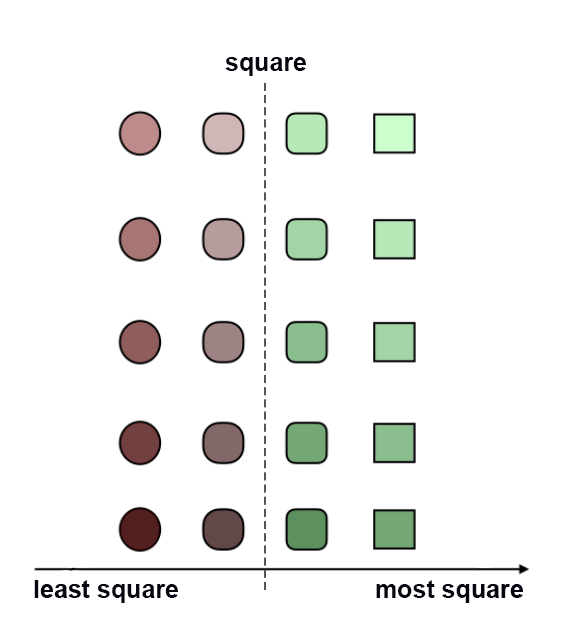
\includegraphics[width=250px]{images/Toyhyperplane1Direction.png}
	\centering
	\caption{An example of a hyper-plane in a toy domain of shapes. The hyper-plane for the word square is the dotted line. Green shapes are positive examples and red shapes are negative examples. Those closest to the hyper-plane are less square than those further away}\label{ch3:HyperPlaneNoDir}
\end{figure}

Linear SVMs obtain a hyper-plane for each model that  separates documents that contain the word and documents that do not contain it. We show an example of this in a toy domain of shapes in \ref{ch3:HyperPlaneNoDir}, where the dotted line is a hyper-plane. As shown in this example, it can be assumed that documents furthest from the hyperplane on the negative side are the least representative of the thing being separated by the hyper-plane, in this case the 'squareness' of a shape, and the documents that are furthest from the hyper-plane on the positive side are the most representative, while those closest to the hyper-plane are more ambiguous. By simply taking the coefficients (orthogonal vector) of this hyper-plane, a direction can be obtained  that goes from documents that are the most distant from the hyper-plane on the negative side, to those that are most distant from the hyper-plane on the positive side (see the direction shown at the bottom of the example in \ref{ch3:HyperPlaneNoDir}).

By measuring how far up a document is on the orthogonal direction vector for a word, a ranking of that document on that word can be obtained, e.g. how 'Funny' it is relative to the other documents. After repeating this process for all documents on a word direction,  features that rank  documents on a a variety of words can be obtained. To get a representation that contains less noise, only those words that are well spatially separated in the representation can be included. This is the first step of the approach described by \ref{Derrac2015} towards re-organizing a document embedding  such that the features encoded spatially are disentangled into  features of the representation. Specifically, first  hyper-planes are obtained for all words based on binary frequency. Then,  words are identified that are semantically important (by e.g. F1 Score or accuracy of the SVM classifier). Finally, orthogonal directions for these word hyperplanes are obtained and  documents are ranked on how far up they are on these directions. These ranking of high-scoring words are then used as the new disentangled representation.

 However, these word labels of directions, although direct, can be ambiguous. For example, in a domain of IMDB movie reviews "numbers" could be referring to musical "numbers" in a broadway musical movie, or the amount of mathematics done by the actors. To resolve this, similar words can be clustered together e.g.  we can give context to the word "numbers" by clustering together similar word directions  "singing songs musical song numbers dance dancing sings sing broadway". This can be done with an off-the-shelf clustering algorithm like K-means (see \ref{bg:clustering}) that uses the word direction vectors as input. We show examples of these word cluster labels for the features of our interpretable representation in \ref{ch3:ExampleRep}.
 
 
 \begin{table}[] 
 	\scriptsize
 	\begin{tabular}{lll}                                                                   
 		\textbf{IMDB Movie Reviews}                                 & \textbf{Flickr-Placetypes}           & \textbf{20-Newsgroups}                           \\
 		\toprule
 		courtroom legal trial court                                 & broadway news money hollywood        & switzerland austria sweden swiss     \\
 		disturbing disgusting gross                                 & fir bark activism avian              & ham amp reactor watts                \\
 		tear cried tissues tears                                    & palace statues ornate decoration     & karabag armenian karabakh azerbaijan \\
 		war soldiers vietnam combat                                 & drummer produce musicians performers & 4800 parity 9600 bps                 \\
 		message social society issues                               & ubahn railways electrical bahn       & xfree86 linux                        \\
 		events accuracy accurate facts                              & winery pots manor winecountry        & umpires umpire 3b viola              \\
 		santa christmas season holiday                              & steeple religion monastery cathedral & atm hq ink paradox                   \\
 		martial arts kung                                           & blanket whiskers fur adorable        & lpt1 irq chipset mfm                 \\
 		bizarre weird awkward                                       & desolate eerie mental loneliness     & manhattan beauchaine bronx queens    \\
 		drug drugs dealers dealer                                   & carro shelby 1965 automobiles        & photoshop adobe                      \\
 		inspirational inspiring fiction narrative                   & relax dunes tranquil relaxing        & reboost fusion astronomers galactic 
 	\end{tabular}  
 	\caption{Example features from three different domains, where each cluster of words corresponds to a direction which movies are ranked on}\label{ch3:ExampleRep}    
 \end{table}   
 
This Chapter builds on the original method to find directions in a document embedding model and rank documents on them introduced by Derrac \cite {Derrac2015}. Specifically, the contribution of this chapter  is an extensive quantitative examination in section \ref{ch3:quantitative} and qualitative investigation in Section \ref{ch3:qualitative} across five domains (as described in Chapter \ref{ch2.5}) and four document embedding models. Variants to  the method introduced in this work are specified in Section \ref{ch3:method}, with the overall goal of the chapter to examine how the new variants perform relative to each other, understand their degree of disentanglement by using simple decision tree classifiers, and verify that the method works in a variety of domains and document embedding models.  Finally, conclusions are made on the contribution of the chapter in section \ref{ch3:conclusion}. %In the next Chapter \ref{ch4} builds on this method by applying and investigating its usage with vector spaces obtained from supervised neural networks, and the Chapter \ref{ch5} identifies problems with this method and introduces a novel unsupervised solution to improve performance.
 

%The original method introduced by Derrac \cite{Derrac2015} used this insight to obtain word-directions, i.e. vectors that go from objects that least have a word to ones that have it most. 

%Conceptual spaces are interpretable vector spaces with features that correspond to key cognitive perceptions of objects, essentially covering the building blocks of the domain. e.g.  in the example of real objects these quality dimensions would be 'temperature, scikit-learn, brightness, pitch and the spatial dimensions of height, width and depth'. In these spaces, instances of objects are points, e.g. "toaster", "house", "fork", and properties e.g. "household-appliances", "buildings" are convex regions. 


 %Conceptual spaces are representations with dimensions intended to represent various "qualities" of objects \cite{Zenker2015} e.g. in the example of a real object we could represent it in terms of 'temperature, scikit-learn, brightness, pitch and the three ordinary spatial dimensions of height, width and depth' \cite{Gardenfors2014}.  

% Ideally, these representations would have dimensions corresponding to clearly defined properties of objects in the domain, e.g. in a domain of IMDB movie reviews, example properties of a movie would be how 'Scary' it is or how 'Funny' it is.

%A representation that models complex relationships and is interpretable could be used in a variety of domains that require interpretability and have difficult tasks, as covered in the previous section \ref{ch2:Interpretability}.


 %The relationships embedded spatially can represent information that is difficult to obtain otherwise. 
 
%We give an example of property-directions in a toy domain in \ref{ch3:toy_domain}.  In this example, there are two property-directions 'light' and 'square', with instances of shapes as points. The instances that have the properties the least are in the bottom left of the direction, and instances of shapes that have the properties the most in the top right. In the IMDB movie review domain, the shapes would be movies, represented as points, and the directions would be properties of movies e.g. how "Romantic" it is, with the least 'Romantic' movies at the base of the direction and those the most 'Romantic' at the tip of the direction. 

%These property-directions give a natural way to obtain an interpretable representation of a vector space. First, property-directions are identified in the space, then a ranking is derived from these property-directions where documents that are lower on the property-direction are given lower ranks, and documents that are higher on the property-direction are given a higher rank. Finally, these rankings are taken as features of a new interpretable representation. 

\section{The Use of Directions in Vector Spaces}

Directions in document embedding models that go from documents that least represent a word, to those that most represent it, can be useful in a wide variety of applications. The most immediate example is perhaps that they allow for a natural way to implement critique-based recommendation systems, where users can specify how their desired result should relate to a given set of suggestions \cite{Viappiani2006}. For instance, \cite{Vig2014} propose a movie recommendation system in which the user can specify that they want to see suggestions for movies that are ``similar to this one, but scarier''. If the direction of being scary is adequately modelled in a document embedding model of movies, such critiques can be addressed in a straightforward way. Similarly, in \cite{Kovashka} a system was developed that can find ``shoes like these but shinier'', based on a document embedding model that was derived from visual features. Semantic search systems can use such directions to interpret queries involving gradual and possibly ill-defined features, such as ``\emph{popular} holiday destinations in Europe'' \cite{Jameel}. While features such as popularity are typically not encoded in traditional knowledge bases, they can often be represented as document embedding model directions.  As another application, directions can also be used in interpretable classifiers. For example, \cite{Derrac2015} learned rule based classifiers from ranks induced by the feature directions.

Other work which has taken advantage of directions in vector spaces has relied on word-embeddings \ref{bg:WordVectors}. For instance,  \cite{gupta2015distributional} found that features of countries, such as their GDP, fertility rate or even level of CO$_2$ emissions, can be predicted from word embeddings using a linear regression model.   In \cite{kim2013deriving} directional vectors in word embeddings were found that correspond to adjectival scales (e.g.\ bad $<$ okay $<$ good $<$ excellent) while \cite{Rothe2016} found directions indicating lexical features such as the frequency of occurrence and polarity of words.








%The way that these features are obtained is by predicting . To  apply this idea to a real domain,  %Although these directions do formally correspond to vectors, we refer to them as directions to emphasize their intended ordinal meaning: feature directions are aimed at ranking entities rather than e.g.\ measuring degrees of similarity. %Graphical representation of 


%\begin{figure}[t]
%	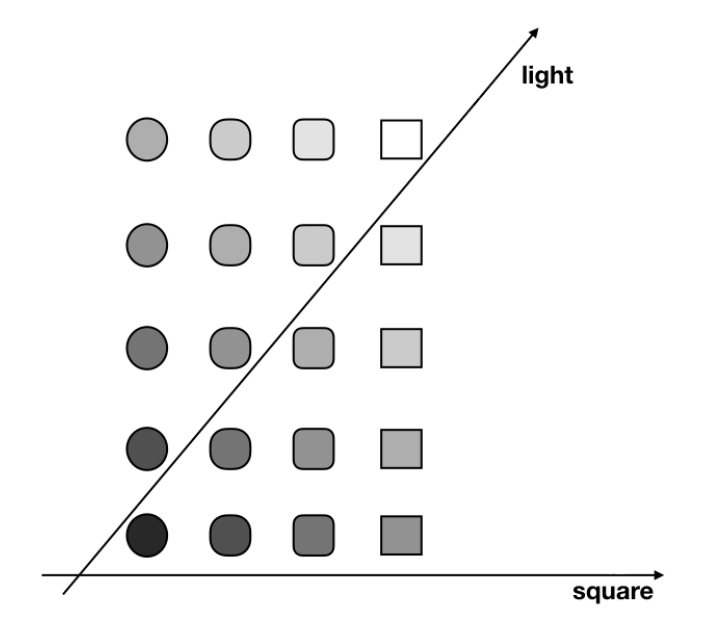
\includegraphics[width=250px]{images/toy_domain.png}
%	\centering
%	\caption{An example of direction in a toy domain of shapes.}\label{ch3:toy_domain}
%\end{figure}



%For example, in a domain using the IMDB movie review dataset, the interpretable features would be labelled with how 'Scary' a movie is, and another that corresponds to how 'Funny' it is.



%This chapter investigates how to make the spatial structure of a semantic space explicit, such that a new representation is formed where each feature models the spatial representation of a property in the domain.
 






%Interpretability as an idea has a variety of interpretations and meanings (See \ref{ch2:Interpretability}). In this thesis, an ideal interpretable representation's features have three important properties: First that each feature models an important aspect of the domain, second that these aspects are distinct from each other, such that each feature represents a unique aspect of the domain, and thirdly that each feature is labelled with a cluster of words describing the aspect of the domain the feature is modelling. The method is entirely unsupervised and 'disentangles' an existing vector space model into salient features. The idea of disentanglement is present in representation learning \cite{Bengio2012} e.g. when given a raw video file of a person jumping, ideally a representation would spatially separate the notions of 'jumping', from the 'person', and the 'background'. In this work disentanglement is used to refer to separating an existing vector space into salient features, such that each dimension of the space is a labelled feature. 




% Why a conceptual space representation? What are entities/properties in that context?

%Perception can be boiled down to objects, or entities. These entities can be described using properties. For example, for the property of "tall", there would be object instances of humans relative to each other on a ranking of tallness. A representation that employs this kind of idea can be known as a conceptual space, where entities are represented as points and spatial relations correspond to properties. 

%What kind-of representation are we introducing? / What is a ranking? How would a ranking on properties be useful? Why is that a good problem to solve?

%How is this representation obtained? 

%How is this representation evaluated?

%Conceptual spaces are a particular way of viewing semantic spaces, where entities (e.g. documents in the case of a document-based representation, or words in the case of word-vectors) are represented as points in the space. Then, properties are aspects of these documents in the space. 

%The spatial structures of semantic spaces have been used in a variety of ways. In \cite{Dai} it was shown that it is possible to perform vector operations on Paragraph Vectors,  e.g. subtracting word-vectors from paragraph vectors, like in the case of a corpus of arxiv papers, a paper titled "Spectral Clustering", could have the word-vector for "Spectal"  subtracted from it to get papers about general clustering. In the case of distributional representations of words \cite{TomasMikolovWen-tauYih2013} found that "equivalent relations tended to correspond to parallel vector differences" \cite{Mitchell2015}, found that by decomposing representations into orthogonal semantic and syntactic subspaces they were able to produce substantial improvements on various tasks.

%The spatial structures we leverage in this work are found in document representations. In particular, directional vectors that describe a particular feature of a domain. Derrac \cite{Derrac2015}  found directions corresponding to properties such as `Scary', `Romantic' or `Hilarious' in a semantic space of movies, for example a direction which goes from a movie that is the least 'Scary' to the most 'Scary'. 

  %The basic idea of this chapter is that we use these feature-directions to produce a representation where each dimension is a ranking of entities on those feature-direction, and evaluate its effectiveness using simple linear classifiers.


% Introduce semantic spaces in the context of using them to produce an interpretable representation



% Explain the previous work

% Explain our work







% These interpretable representation are demonstrated to be effective in simple linear classifiers on document classification tasks. 




 %The intention of this work is to produce interpretable representations and simple interpretable classifiers that use the domain knowledge spatially encoded by any learning method. 
%Interestingly, the method can even be used to obtain an interpretable representation from neural networks, as they learn vector space models as hidden layers, which is investigated in Chapter \ref{ch5}. %as hidden layers have achieved state-of-the-art results in a majority of NLP tasks e.g. learning using large amounts of data, transferring that data between tasks, or integrating additional constraints.
%in particular those based on the distributional hypothesis have become commonly used in many state-of-the-art natural language processing models, and have been augmented and improved in a variety of ways. For example, Distributional word vectors have achieved state-of-the-art in Language Modelling by ensuring frequent and rare words are given similar semantic importance \cite{Gong2018}, 



%%%% Build up the variance in space types and how they are produced 
%There are many ways to produce a Vector Space Models, from frequency statistics using dimensionality reduction methods like PCA or MDS, to applying the distributional hypothesis and learning through word context, to learning neurally with structural or supervised constraints, e.g. enforcing hierarchical grammar, or integrating different kinds of data, e.g. image data. This has resulted in a wide variety of spatial structures in these representations, each one suited to certain tasks or domains. These representations, in particular distributional and neural representations have recently found widespread success in many domains, e.g. X, Y, Z. 

% (e.g. natural clusters form like in a domain of movie reviews, movies of a positive sentiment would be in a cluster distinct from those of negative sentiment)
%These concepts are instead embedded in the spatial relationships of the space. This has lead to work in understanding exactly how these spatial relationships correspond to domain knowledge. There are many approaches to understanding Vector Space Models, from visualization and exploration tools enforcing sparsity constraints on existing methods, e.g. on distributional vectors using NNSE or with sparse-PCA, to neural network models that produce an interpretable representation e.g. InfoGan is able to produce a representation where each dimension corresponds to an aspect of a handwritten digit, with one dimension for style and so on, or other networks or finding clusters or labelling existing dimensions. However, in this case we are interested in a linear transformation of any existing Vector Space Model. This is a representation agnostic approach, which is valuable as it can make use of the structures already developed for whatever representation is suitable for our task. The benefit of this can even extend to interpreting the 'hidden layers' of supervised networks, as seen in Chapter 5. The second benefit  our method has is that it is entirely unsupervised, and by ensuring that salient semantics of the space are used as features for the new representation we are able to produce simple interpretable linear classifiers, in this case the interpretability of these classifiers being defined as using our interpretable features as components. We show an example of a tree using such features below.

%example nne, nnse, or for frequency statistics sparse pca. In terma of functionality, we coiod compare our method to obtaining a specialized topic model, as both contain labelled features - with the main difference being topic model representations are induced probabilistically rather than inducing a Vector Space Model. We show a comparison between the best performing topic model topics (LDA, see \ref {ch2:LDA}) and our method below.

%In this chapter, we experiment with a method to produce an interpretable representation from an existing Vector Space Model and its associated Bag-Of-Words by leveraging its spatial relationships. This approach gives us a number of benefits. First, we are able to leverage a variety of different Vector Space Models according to the problem that needs to be interpretably solved. Second, we can transform the space in an entirely unsupervised way without needing additional data or supervision signals. 

%The simple linear interpretable classifiers we can obtain from our method are low-depth Decision Trees. if those dimensions correspond closely to the classes we intend to solve (e.g. classifying if a movie is a horror wouls only require a single dimension tp be used in the classifier, and would resolve many desirable properries e.g. generalization.

%in parare useful for our method because unlike a Bag-Of-Words, they encode how these words relate to each other, form the greater concept of a 'Horror' movie, and how the movies which contain these words relate to each other. This kind of knowledge is beneficial to complete knowledge bases, and to capture more complex relationships that can correspond to fuzzy and commonsense knowledge about documents,

%The origin of our method is in commonsense reasoning. The structure of Vector Space Models have been shown to contain properties of commonsense reasoning,  e.g. where movie reviews are documents analogical relations (scary movie 1 is to scary movie 2 as harry potter and the philosophers stone is to harry potter and the chamber of secrets), commonsense betweeness (movies age rated 15 would be spatially between those rated 18 and those rated 12), and so on. These are the kind of semantic relationships we leverage to obtain our representation.

%The method transforms the space into an interpretable representation built on the spatial relationships of the original space. 



%e give an example of the dimensions of a 'disentangled' representation in \ref{ch3:disentangled}. and our experiments in this chapter focus on the performance of a disentangled representation in this context. Further, the methods we investigate are entirely unsupervised, needing only a Bag-Of-Words and an existing Vector Space Model. 

%Interpretable models are generally in three categories, 
%But these topic models do not contain the rich spatial relationships found in Vector Space Models, and their representations cannot be augmented by additional data or grammatical information in exactly the same way.  %Frequency statistics and distributional neural embeddings like word-vectors have achieved strong performance on X by doing B, Y by doing N, Z by doing K. 
%For example, a good vector space in the domain of movies constructed from IMDB movie reviews should contain a natural separation of entities into genres, where Horror movies are spatially distant from Romance movies, and movies that are Romantic Horrors would be somewhere inbetween. We can see an example in Figure \ref{figure:genres_separated}. For a Bag-Of-Words, we can expect similar entities to have similarly scoring terms \ref{PPMI table:PPMI_example}.

%\begin{figure}[t]
%	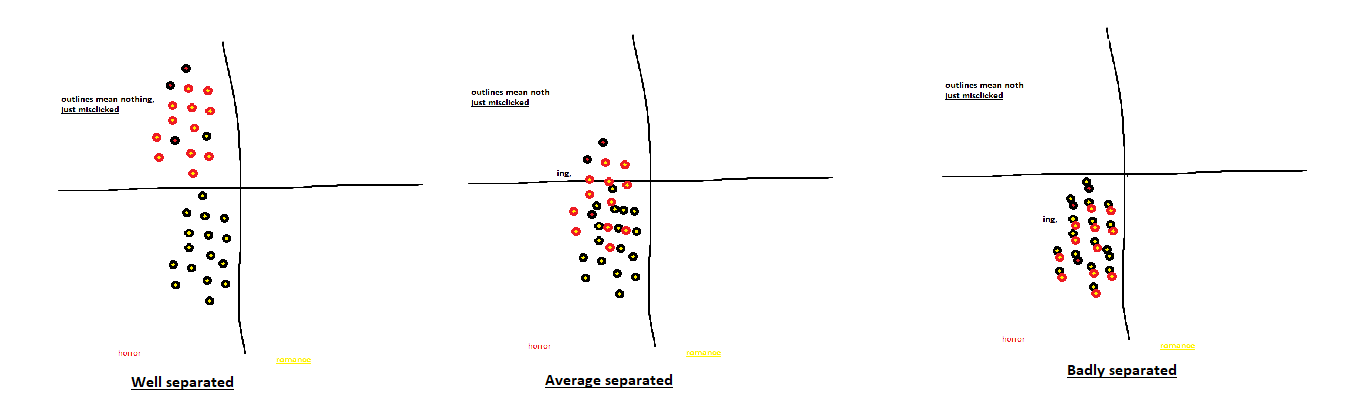
\includegraphics[width=\textwidth]{images/genres_separated.png}
%	\centering
%	\caption{A conceptual space of movies, where regions correspond to properties and entities are points.}\label{figure:genres_separated}
%\end{figure}

%The relationships in Vector Space Models can be extracted to obtain domain knowledge. %king and queen was parallel to the vector between prince and princess. % NEED TO MAKE THIS REAL


%The simple  classifiers that are used to evaluate the method's feature directions are low-depth Decision Trees. In Figure \ref{ch3:DecisionTree} an example is shown of a shallow Decision Tree using the method's interpretable representation. Shallow Decision Trees were chosen because they are effective at evaluating the disentanglement of the representations features. If the features are disentangled, then a low-depth Decision Tree will suffice to classify natural domain tasks. Shallow trees also evaluate the semantic generalizability of the features, as if they are able to classify complex classes using only a single feature then that feature must be semantically coherent and generalizable.% In terms of interpretability, shallow trees have many positive effects for users, like lower response times \cite{Narayanan2018, Huysmans2011}, better question answering and confidence for logical problem questions \cite{Huysmans2011} and higher satisfaction \cite{Narayanan2018}. Although in this work  the superiority of  low-depth Decision Trees in real-world interpretability applications is not in the scope of the evaluation, as the interpretable representations  could be applied to a variety of classifiers.

%The quantitative results for the method show that the method can successfully disentangle a variety of representations even with trees as limited as depth one, and these shallow trees outperform the original representation greatly when compared to deeper trees on the uninterpretable original features. Additionally, the results in most cases are also competitive with Latent Dirchlet Allocation, a baseline interpretable topic model. The method is shown to be an effective way to obtain a disentangled representation that can effectively produce simple interpretable classifiers. The method is verified to work on five different representation types for five different domains, using natural domain tasks for those domains. 



%Why interpretability for document classification matters:

%What Vector Space Models are there that perform well at tasks:

%What document classification tasks are important:

%What methods are there for interpretable document classification:

%Derrac \cite{Derrac2015} introduced an unsupervised method to go from a Vector Space Model and its associated Bag-Of-Words to a representation where each dimension is a ranking of documents on a feature of the domain. For example, in the domain of movie reviews genres would be a feature, and the dimension would have a numeric value for each document corresponding to the degree it is a particular genre. The contribution of this Chapter is an analysis and experimentation on the quality of these features applied to document classification. The main insight from our work is that these interpretable features do not suffer a performance drop in a non-linear classifier compared to the original representation, and can outperform the original representation and a baseline interpretable representation in a linear classifier. In addition, we find that if a dimension ranks documents on a feature relevant to the task, it can be competitive with more complex models using a single Decision Tree node. We show an example of the representation from a domain of IMDB movie reviews in \ref{ch3:TreeAndRep}. 

%\begin{figure}[t]
%	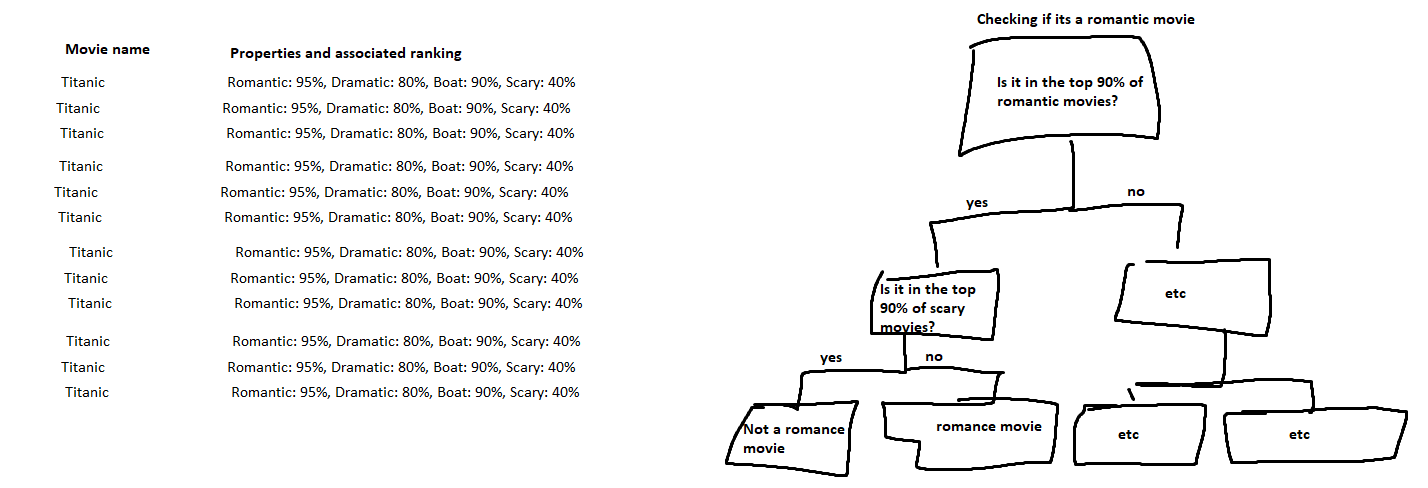
\includegraphics[width=\textwidth]{images/tree and rep.png}
%	\centering
%	\caption{Example movies and selected associated dimensions, chosen according to their relevance to the genre task.}\label{ch3:TreeAndRep}
%\end{figure}

%Vector Space Models encode semantic relationships

%What are the applications of semantic relationships? What is the power of a semantic relationship? Why are semantic relationships important in a space?
%prolly need more about

%What are directions? Why are directions important? What have they been used for? What is a feature direction?


% How can I apply directions to produce an interpretable space? Why is this valuable? What makes this interesting? What are feature rankings?


%%What are the advantages, disadvantages of the previous work?



%Why do this work? What is the value of this work?  How is this relevant to the readers interests?


%\subsection{Using a Property Representation in a Linear Classifier}


%Our method can use any vector space that linearly separates entities, and so it has potential longevity. This means that our method is relying on structure in the space that does not directly correspond to our desired representation -  we can view our approach as a linear transformation of the space. We address this problem in Chapter \ref{chapter:finetuning}. However, we have the capability to leverage many different methods to construct a vector space for our representation, so as long as dense representations of entities exist it will be possible to use our method, and as they are improved the results that our method can achieve will be improved too. This kind of flexibility also gives us the potential to combine the resultant representations from different vector spaces for classification, e.g. concatenating the vectors from different spaces.

%Topic models such as Latent Dirichlet Allocation (LDA) represent documents as multinomial distributions over latent topics, where each of these topics corresponds to a multinomial distribution over words \cite{Blei2003}. These topics tend to correspond to semantically meaningful concepts, hence topic models tend to be rather interpretable \cite{Chang2009}. To characterize the semantic concepts associated with the learned topics, topics are typically labelled with the most probable words according to the corresponding distribution. 

% What is a Vector Space Model? Why is a Vector Space Model valuable?




% 




%%What is the previous work?
 %What is a direction




%Finally, \cite{derracAIJ} found salient properties as direction vectors in a Vector Space Model of entities (e.g. Movies in a domain of IMDB movie reviews), and labelled them with clusters of words (e.g. $p_1 = {Scary, Horror, Gore}, p_2 = {Funny, Laughter, Hilarious}$).  We show a toy example in Figure \ref{ToyDirection}. %Copied from CONLL 




%%What is our contribution towards those disadvantages in this chapter?
%"Decision Trees, Decision Tables and Textual descriptions of rules are logically equivalent in the sense that one type of representation can be automatically translated to another (albeit in a simpler or more complex form), while preserving the predictive behaviour of the original model"


%%What are some real world scenarios that you could see our work taking effect in?
%In a case study by , giving the business users the option between a model with higher classification score but more input variables and a lower classification score but less input variables resulted in more buy-in for system designers. By accurately representing salient concepts in the domain, we are also able to offer a similar option; less nodes in the Decision Tree in exchange for more accuracy. % Potentially this citation sucks


%How is the work evaluated? How can you justify the evaluation? 
%%What are some alternative interpretable classifiers? What are some approaches to interpretable classification?

%%How does our work fit into the niche of interpretable classifiers?

%%What kind of tasks are these interpretable classifiers usually on? How do we compare in terms of evaluation?

%%How does our evaluation of interpretability play into our idea of interpretability outlined in Chapter 1?





%Broadly speaking, in the context of document classification, the main advantage of topic models is that their topics tend to be easily interpretable, while Vector Space Models tend to be more flexible in the kind of meta-data that can be exploited e.g.\ they allow us to use neural representation learning methods to obtain these spaces. The approach proposed in this Chapter aims to combine the best of both worlds, by providing a way to derive interpretable representations from Vector Space Models.  

%Topic Models are also entirely probabilistic, while our method relies entirely on the spatial relationships present in the vector space model.



%How is the chapter going to play out? Whats going to happen?
%As our work performs well even at lower-depth trees, this gives potential users more flexibility in how they want to present the information, e.g. to a potential client. Compared to Bag-Of-Words, which loses its representation capabilities the lower the depth.

%This chapter continues as follows: First the method is described, . This is followed by a qualitative  and quantitative analysis, finishing with a conclusion on the  benefits and limitations of this approach.



%\section{Related Work}
%Sparse word vectors
%Adapted to composition \cite{Fyshe2015}
%\subsection{Semantic Relations \& Their Applications}

%Our method uses the relationships inherent in a Vector Space Model. Other work has formalized the relationships found in Vector Space Models, for example in word-vectors, linear analogies (see Section \ref{WordVectors, Ethayarajh2018}, were found where the vector between  %Copy pasted from this 
%[ENTIRE SECTION COPY PASTED FROM PREVIOUS PAPER]
%\textbf{Linear Classifiers}
%Decision Trees, linear SVM's, logistic regression, decision tables, IF Then rules.

%What are the available options for interpretable linear classification?

%How have each of these methods been measured or validated in the literature in regards to interpretability? How about application to real world situations?

%\textbf{Non linear classifiers}
%What non linear classifiers networks are interpretable? How have they done it? How have they measured it? How does it compare to a linear method?

%\textit {Neural networks}Approximating w/linear model, Interpretable nodes/weights

%\textit {Other Stuff}

%\subsection{Interpretable Representations}


%There are two ways in which topic models can be used for document classification. First, a supervised topic model can be used, in which the underlying graphical model is explicitly extended with a variable that represents the class label \cite{Blei2010}. Second, the parameters of the multinomial distribution corresponding to a given document can be used as a feature vector for a standard classifier, such as a Support Vector Machine (SVM) or Decision Tree. .




% One of the more popular models for text representation that labels features in a similar way to our method are Topic Models.

\section{Background}\label{ch3:background}

\section{Clustering}\label{bg:clustering}

\subsection{K-means}

% USING DEFAULT PARAMETERS NOW

\subsection{Derrac's K-means Variation}


\section{Method}\label{ch3:method}
% Assumed understanding at this point
% Chapter 1: Why interpretability is important. The value of a good interpretable representation. What directions are and what they mean.
% Chapter 2: The background and literature review for interpretable representations.
% Chapter 3: An introduction on the value of a good interpretable classifier, and the position of our work in that domain and how it can be applied there. What entities, properties are. What a conceptual space is. A literature review on relevant interpretable classifiers.

This section details the methodology to disentangle a document embedding model starting with only itself and its associated Bag-Of-Words \ref{bg:SemanticSpaces}.  The work in this chapter differs from the method introduced by Derrac \cite{Derrac2015} as it focuses on investigating the quality of these disentangled representations using simple  classifiers. Multiple variations are introduced and included as part of the experimental method.%which whose features rank documents on salient semantics, e.g. In a domain of IMDB movie reviews, a movie would be ranked on semantics like  $1: \{Scary, Horror, Bloody\}$ and $2: \{Romantic, Love, Cute\}$, ideally with as many rankings as salient semantics of the domain. 
%Make sure features ae explained well earlier 

%\subsection{The Structure of a Vector Space Model}

%Salient features of the domain are encoded in the structure of a Vector Space Model. 
% What are directions? How are they encoded? Why are they encoded that way?

%%%%%%%%%%%%%%%%%%%!!!!!!!!!!!!!!!!!!!!!!!!!!!!!!!!!!!!!!!!!!!!!!!!!!!!!!!!!!!!!!!!!!!!LOOK HERE
% Convert to table
%word: $w$

%document $d$

%vector-space of documents $V_d$ where $d = (x_1, x_2, ..., x_n)$ where $x$ are features and $x(d)$ is equal to the value of a feature for a document

%bag-of-words of documents $B_d$ where $d = (wf_1, wf_2, ..., wf_n)$ and $wf(d)$ is equal to the frequency of that word in a document and $n$ is equal to the number of unique words across all documents.


%model for a word ($M_w$)

%hyper-plane for a word = $H_w$

%orthogonal direction vector = $\mathcal{D}_w$

%ranking of all documents on a word direction  $R_w = ({rw}_{d1}, {rw}_{d2}, ..., {rw}_{dn})$ where ${rw}_{d}$ is equal to the ranking of a document on a word direction

%cluster of words $C = (w_1, w_2, ..., w_n)$

%cluster direction = $\mathcal{D}_C$

%interpretable representation composed of rankings $I_d$ where $d = (R_{w1}, R_{w2}, ..., R_{wn})$ and $R_w(d)$ is equal to the ranking of a document on a word direction

%interpretable representation composed of cluster rankings $I_d$ where $d = (R_{c1}, R_{c2}, ..., R_{cn})$ and $R_c(d)$ is equal to the ranking of a document on a cluster direction

%ranking of documents on direction
 
 %%%%%%%%%%%%%%%%%%%!!!!!!!!!!!!!!!!!!!!!!!!!!!!!!!!!!!!!!!!!!!!!!!!!!!!!!!!!!!!!!!!!!!!LOOK HERE

%\begin{figure}[t]
%%	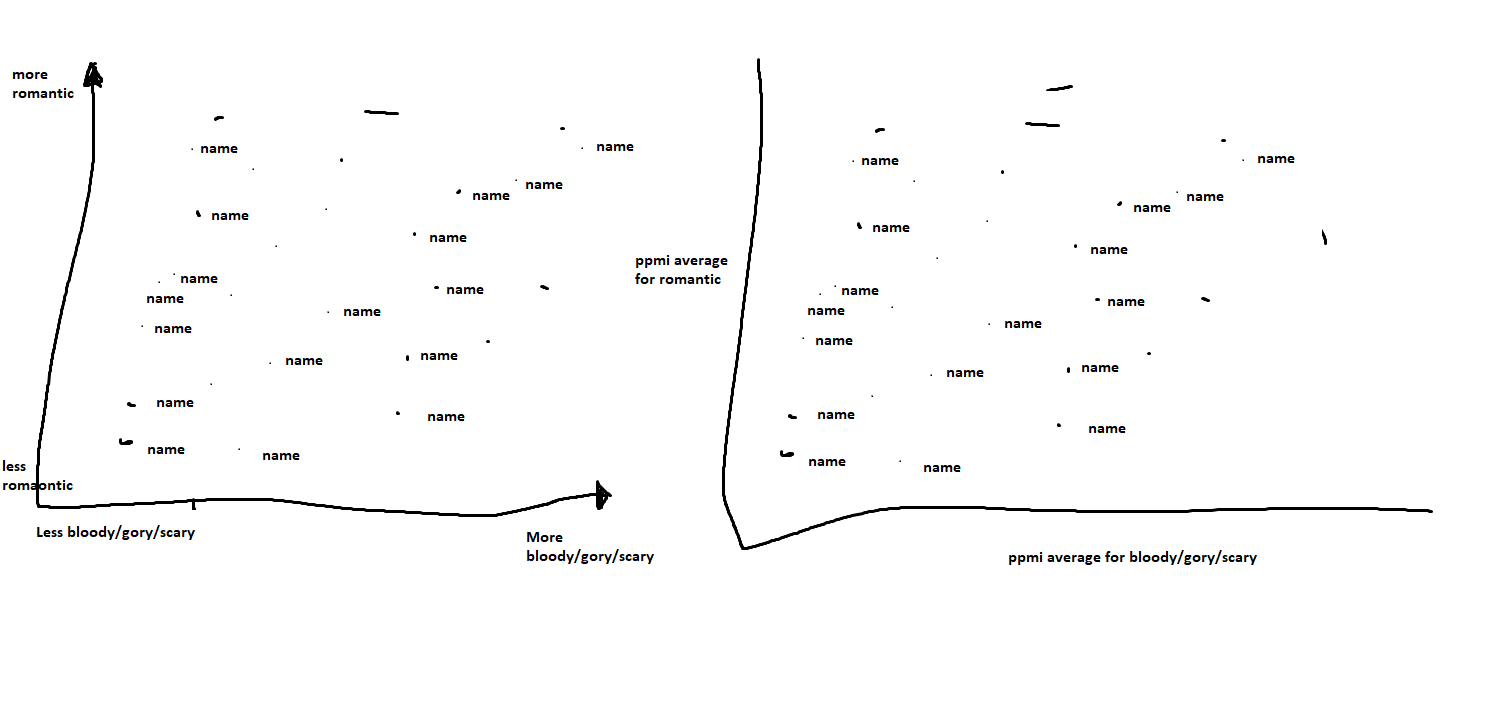
\includegraphics[width=\textwidth]{images/DirectionsGraphic.png}
%	\centering
%	\caption{Original And Converted.}\label{ch3:DirectionsGraphic}
%\end{figure}
%The method to obtain interpretable feature-vectors is an extension of the work by \cite{derracAIJ}. This previous work showed how to, filter out words, cluster words to get features, and obtain rankings of documents on those features. In this section, we further analyse and extend this work, in particular by testing a variety of additional filtering methods and clustering methods, and demonstrating how these feature-vectors can produce simple linear interpretable classifiers. 
%To begin, we filter out terms that will not be well represented in the space, and in-turn will not result in good feature rankings. We do so by first removing all terms below a frequency threshold. Then, for each word we obtain a direction in the space that can induce a ranking of documents on that word, and evaluate how well represented that word is in the space and remove those below a threshold. We can consider the terms remaining to be candidate feature-directions, as they are all well represented in the space and are unlikely to be highly scored as representative due to being infrequent. However, it is possible that they may not represent different information from each other, e.g. "blood" and "bloody" are likely quite similar. Additionally, we can understand that a good feature will not correspond directly to a term, but instead to a more abstract concept, e.g. "Blood, Gore, Horror". To obtain these more abstract feature-directions, and ensure the feature-directions are distinct rather than representing the same information, we cluster together similar feature-directions and obtain their feature-rankings to obtain our final representation. Each of these feature-rankings can be labelled with the cluster of words they are composed of. 



\subsection{Obtaining Directions and Rankings From Words}\label{ch3:LearningInterpretableDirections}

 The method starts with a given document embedding  induced from text documents $D$ and their associated bag-of-words $B$. The bag-of-words representation of a document $d$ is given by its vector of word frequencies $b = (\textit{wf}_1, {wf}_2, ..., {wf}_n)$ where ${wf}(d)$ is equal to the frequency of a word in a document and $n$ is equal to the number of unique words  in the vocabulary $W$.
  Following the general explanation in the introduction, this section more precisely explains how to obtain a word-direction vector $\mathcal{D}_w$ for all words in the vocabulary $w \in W$, by using a vector found by a linear model $M_w$ that separates documents that have a word and do not have a word. Then, from that direction it explains  how to obtain a ranking of all documents $R_w = ({rw}_{d1}, {rw}_{d2}, ..., {rw}_{di})$ where ${rw}_{d}$ is equal to the ranking of a document on a word direction and $i$ is the number of documents. The section following this one shows how to remove word directions that are not semantically important by evaluating the quality of the classifier that obtained the direction $M_w$, or the quality of the direction $\mathcal{D}_w$.


%%%%%%%%%%%%Features that are important will be spatially organized in a way that reflects the similarity between the Bag-Of-Words representations they were composed of. In particular, we expect that documents will be arranged in a direction, where generally the higher the PPMI score for a group of words that correspond to a feature (e.g. $Horror, Scary, Gore$) the further away they will be from those that have low PPMI scores for those words. We give examples of this in Figure \ref{ch3:DirectionsGraphic}, by projecting documents into a 2D space of salient features we are able to show that these documents are structured according to directions for these features. Salient features will typically be a more abstract representation which will be natural in the domain, e.g. in a domain of IMDB movie reviews, genres

\noindent \textbf{Obtaining directions for each word} Each document is represented by a vector $v_d $ in the document embedding model $V_D$. %For this section, document vectors $v_d$ are treated as points $p_d$ in the document embedding model. 
For each word $w$, a hyper-plane $h_w$ is obtained by training a linear classifier$\footnote{Tested using a logistic regression classifier and a linear SVM, both achieved similar results}$ $M_w$ on the document vectors  so that all documents where the word $w $ occurs more than once are separated from those where the word did not occur. We obtain such hyperplanes for  words in the vocabulary above a frequency threshold ${wf}(D) > T$ where ${wf}(D)$ is the frequency of the word $wf$ in all documents $D$. %In practice, the parameter $T$ is determined with hyper-parameter optimization. 
This task is unbalanced, i.e. there are typically fewer documents that contain the word compared to those that do not contain it. For this reason, the weights of the training examples are weighted, where the weights of the classifier are balanced such that positive instances are weighted in proportion to how rare they are.\footnote{ \href{https://scikit-learn.org/stable/modules/generated/sklearn.utils.class_weight.compute_class_weight.html}{Using scikit-learn, class\_weight:'balanced'}}



Although the hyperplane $h_w$ is classifying a binary class (either classifying documents $d_p$ as negative or positive), the distance between the document vectors $d_p$ and the hyperplane $h_w$ will vary. For example, when separating documents based on the occurrence of a word, it can be expected that the documents which contain the word more frequently would be further away from the hyper-plane on the positive side. We give an example of two directions in Figure \ref{ch3:ToyHyperPlane}. To  apply this idea to a real domain, we can give an example from movie reviews, where the word is 'Scary' and the most 'Scary' movies are at the tip of the direction and those that are least 'Scary' are at the base of the direction. With this understanding, the direction $\mathcal{D}_w$ can be obtained by simply taking the vector perpendicular to the hyperplane $h_w $. This direction goes from documents $d_p$ from those lowest on the direction (at the distance furthest from the hyperplane on the side where documents $d_p $ are classified) to those highest on the direction at the distance furthest from the hyperplane at the positive side. 


 %Although these directions do formally correspond to vectors, we refer to them as directions to emphasize their intended ordinal meaning: feature directions are aimed at ranking entities rather than e.g.\ measuring degrees of similarity. %Graphical representation of 

\begin{figure}[t]
	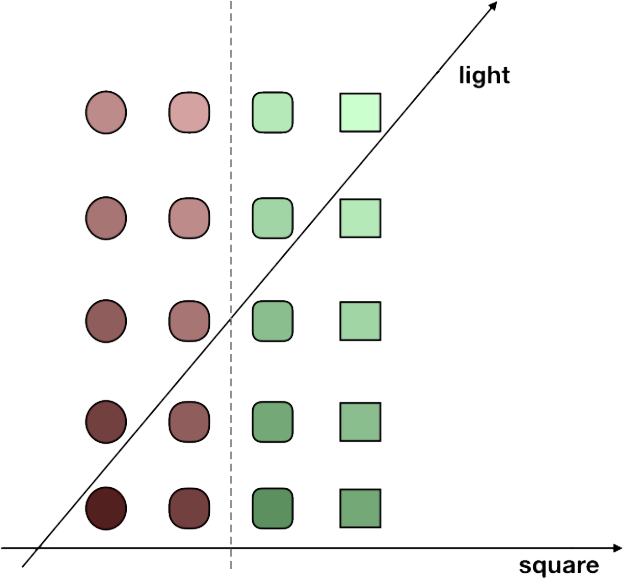
\includegraphics[width=250px]{images/ToyHyperplane.png}
	\centering
	\caption{Another example of a hyper-plane in a toy domain of shapes. Here we show multiple directions, one for light and one for square The hyper-plane for the word square is the dotted line. Green shapes are positive examples and red shapes are negative examples for the word square. }\label{ch3:ToyHyperPlane}
\end{figure}


\noindent \textbf{Ranking documents on directions} In this section we specify how to obtain a ranking $R_w$ of all documents on a word direction vector $D_w$. The rank of a document $d$ can be defined by the dot product $\mathcal{D}_w \cdot p_d$ as the ranking ${rw}_{d}$ of the document $d$ for the word $w$. Specifically, ${rw}_{d_1}$ is ranked higher than ${rw}_{d_2}$ if  ${rw}_{d_1} < {rw}_{d_2}$. These rankings measure how relevant the document is in the spatial representation for the word, rather than just frequency e.g.  a document that contains the word "scary" but isn't a scary movie (e.g. if it contained sentences like "it's scary how much money is spent on advertising movies like this") would not be ranked highly on the direction for 'scary', as the word 'scary' is not semantically important for the document. To put it another way, intuitively it can be understood to mean that the document $d_2$ 'has' the feature  to a greater extent than $d_1$, e.g. in a domain of movie reviews if a movie ranked highly on the word 'dull', the movie has more dullness than lesser ranked movies. %Ranking all documents on a word results in a feature that ranks documents on how well they represent that word in their spatial representation.   By obtaining a ranking of all documents for all words,  a feature matrix of size $D_n \times W_n $ is obtained, which is a representation that has a feature for every word in the vocabulary.


In this section, the methodology to obtain word-directions and their associated rankings was described. These word-rankings are useful as features, and hypothetically we could obtain a representation that has as many features as there are words. However, some words are more semantically important in the domain than others. The next step describes how to remove word directions that are not well predicted by the linear model $M_w$, under the assumption that if they are not spatially important (i.e. easily separable), they are not semantically important. Another problem with word-rankings is that their meaning can be unclear, e.g. the word "serial" could be referring to a series of movies, or a "serial" killer\footnote{The real cluster of words that this example comes from  is "gore gory bloody blood gruesome serial investigate deaths"}. To solve this problem, the final section explains methods to cluster words together. This finally results in a representation where each feature is semantically important and has an associated cluster of words to give context. We gave examples of these clusters of words in the introductory table \ref{ch3:ExampleRep}. %To give an understanding of these rankings and their saliency, we show some examples of features and documents ranked on them for different domains with varying degrees of saliency. In the next section, we show how we measure the saliency of directions and filter those that are not salient out of the representation. %Graphical representation of entities being ranked on a direction vector






%\begin{figure}[t]
%	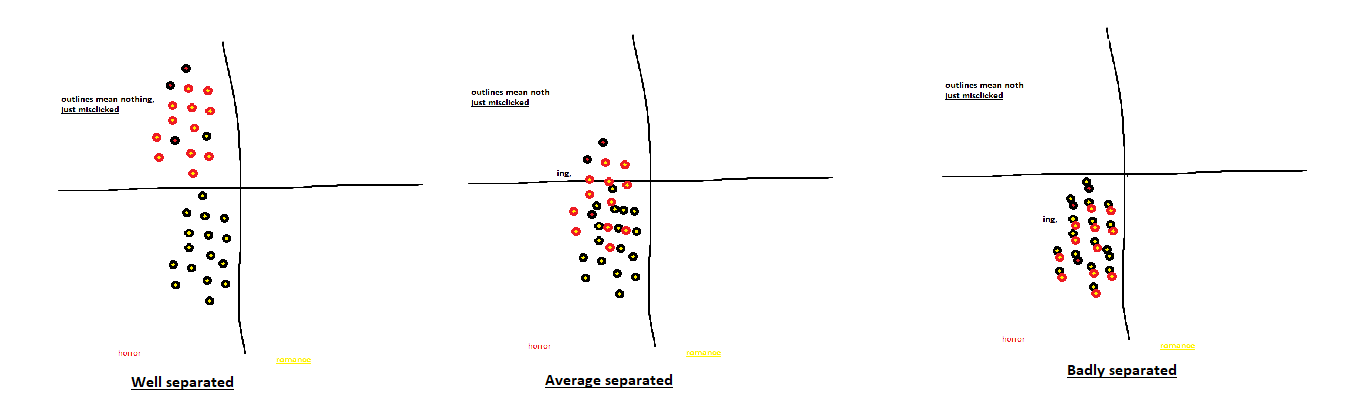
\includegraphics[width=\textwidth]{images/genres_separated.png}
%	\centering
%	\caption{Original And Converted.}\label{ch3:OrigAndConverted}
%\end{figure}



\subsection{Filtering Word-Directions}

%With the rankings $R_r$, we could create a representation of each document $d$, composed of $w_n$ dimensions, where each dimension is a ranking of the document $d$ on that word $r_dw$. However, many of the words are not spatially important enough in the representation to result in a quality ranking - they are not salient features.

% Change to good directions are feature directions 
Although we are able to obtain word directions for every word, not every word is semantically important in the document embedding model. Here, we distinguish between word-directions $\mathcal{D}_w$ as directions that are not semantically important in the document embedding model, and feature-directions $\mathcal{D}_f$, which are. We define the set of feature directions as $f \in F$. Additionally, we make the distinction between a word-ranking $R_w$ which is a ranking on a word-direction and a feature-ranking which is a ranking on a feature-direction  This section how to filter out word-directions so that only feature-directions remain, in-order for the final representation to be composed of only feature-rankings. Additionally, we refer to the word or cluster of words associated with a feature-ranking as a feature-label for that ranking.
 
The assumption made by Derrac in the original work \cite{Derrac2015} was that if a classifier $M_w$ does not predict the occurrence of a word in a document in its embedding well, it is not semantically important. Put another way, if the documents are separated well, it must mean that the word $w$ being used in the description of $d$ is important enough to affect the document embedding model representation of $d$. The occurrence of a word in a document can be evaluated by using a variety of scoring metrics to determine the performance of the classifier $M_w$. This work also introduces a the use of a scoring metric that evaluates the quality of the direction $\mathcal{D}_w$, as even if the documents are well separable, then the ranking induced from the direction may not be correct. This metric compares how well the ranking induced by the hyperplane correlates with a BoW representation. If the ranking does correlate, it can be assumed that this means the word was strongly influential in the document embedding model, as the detail of the Bag-Of-Words information is embedded in the document embedding model's structure. 

After scoring the words using one of the aforementioned metrics, a simple cut-off is applied where the top scoring words are taken as feature-directions (e.g. the top 2000 scored words). By obtaining these feature-directions, we can rank documents on each of them and use them as features of a  representation $I_{Fr}$ where ${Fr} = ({fr}_{d1}, {fr}_{d2}, ..., {fr}_{dn})$ and ${fr}_d$ is the ranking of a document on a feature-direction. In this representation, each feature is semantically important, however there may be overlap, e.g. the word "Gore" and "Gory" likely have similar rankings. Ideally, the score cut-off would be at the point where the words stop corresponding to semantically important features. However, it is difficult to determine this, so in practice this value is taken as a hyper-parameter determined by a classifier on some domain task.

\noindent

\noindent \textbf{Cohen's Kappa}. This is the only metric used in the work by Derrac \cite{Derrac2015}. This metric evaluates the performance of the classifier, and also deals with the problem that these words are often very imbalanced. For very rare words, a high accuracy might not necessarily imply that the corresponding direction is accurate, as if there are a large number of negative examples (as is the case with infrequent words) the classifier could simply predict that all documents do not contain the word to achieve a high score. For this reason, they proposed to use Cohen's Kappa score instead. In our experiments, however, it was found that this can be too restrictive, allowing us to sometimes obtain better results with the more simple accuracy metric.\smallskip %This is basically copy pasted.


 \textbf{Classification accuracy}. If a model has high accuracy for a word $w$, it seems reasonable to assume that $w$ describes a salient property for the given domain. However, despite balancing the weights of the original SVM used to obtain the hyper-plane, the value this metric places on correctly predicting negative classification  compared to Kappa, it might favour rare words as it tends to be easier to obtain a high accuracy for these words.%often results in noise particular to this metric being identified, e.g. metadata like a reviewers name that only occurs in a few reviews being given a high accuracy score as the method, as it overfit to only predict negative instances.%This is basically copy pasted.
\smallskip


\noindent \textbf{Normalized Discounted Cumulative Gain}\label{ch3:NDCG} % MATHEMATICS NEEDS TO BE REWRITTEN 
This is the metric chosen to evaluate the quality of the rankings induced by the direction $R_w$. In-order to do so, two rankings are compared: one defined by the rankings and one defined by PPMI scores.  The metric found to work best was Normalized Discounted Cumulative Gain (NDCG) which is a standard metric in information retrieval that evaluates the quality of a ranking w.r.t.\ some given relevance scores \cite{jarvelin2002cumulated}.  NDCG is mostly affected by the ranking position of the documents for which PPMI is highest.  Spearman Rho, Gini, and Kendall Tau as alternative metrics  do not favour higher ranked documents as much, but this comes with two problems. First, PPMI (See section \ref{bg:ppmi}) leads to a large number of zero scores. If we assume that all documents that have a zero frequency are ranked the same, then the dot products rankings will be greatly different for lower-ranked documents as they instead are ranked according to their spatial representation. This disrupts the score too much to be useful when lower ranked documents are given equal importance to higher ranked ones. In this case, the rankings $R_w$ of the document $d$ are those induced by the dot products $\mathcal{D}_w \cdot p_d$. The relevance scores are determined by the Pointwise Positive Mutual Information (PPMI) score $\textit{PPMI}(w,d)$, of the word $w$ in the BoW representation of document $d$ (See section \ref{bg:ppmi}), under the assumption that they correspond to a good baseline for what we consider to be important for an entity. 
% Taken directly from the journal paper
\begin{align*}
\text{DCG}_{R}^{w} &= \sum_{i=1}^{{pr}_d}\frac{\textit{ppmi}_{i}^{w}}{log_{2}(i + 1)} \\
\text{IDCG}_{R}^{w} &= \sum^{|\textit{documents}|}_{i=1} \frac{2^{\textit{ppmi}_{i}^{w}}-1}{log_{2}(i + 1)} \\
\text{nDCG}_{R}^{w} &= \frac{\text{DCG}_{R}^{w}}{\text{IDCG}_{R}^{w}}
\end{align*}  

To define NDCG, we can first define Discounted Cumulative Gain (DCG), where ${prw}_{d}$ is equal to a position in the ranking of documents on a direction $\mathcal{D}_w$, and $ppmi_{p_{i}}^{w}$ is equal to the PPMI score for a word at position $i$ in the ranking. Then, we can define the Ideal Discounted Cumulative Gain (IDCG), which is the best possible DCG for a position ${prw}_{d}$, where $|documents|$ are the documents for the term ordered by their relevance up to position ${prw}_{d}$. nDCG is then simply the DCG normalized by the iDCG.
  %Below, we show the top 20 highest scoring properties that are not in the top 100 properties when using the other scoring method. As there are a few duplicates between both methods, this is simply to highlight the different kinds of properties each one obtains.
%We show the top scoring terms found by each scoring type below in Table \ref {X}.

\subsection{Clustering Features}\label{ch3:LabellingWords}
A representation composed only of rankings of single words could be used, however that comes with two issues when classifying with a simple  classifier. The first is that there may be too many dimensions, so a  classifier like a Decision Tree (See Section \ref{bg:trees})  needs to be deep to classify well. The second is that it can sometimes be ambiguous what a feature-ranking means when it is labelled with only a single word, e.g. the word "courage" has an associated feature-direction, but what that feature direction represents can only be understood in the context of a cluster of similar words "courage students teaches student schools teacher teach classes practice training learning overcome conflict teaching" showing that it is about courageous teachers and students overcoming challenges. The most naive way to obtain a cluster like this is to find similar word-directions: 

\noindent \textbf{Similarity Labelling} As a way to add context to single word directions, for each single word direction $w \in D_w$, the cosine similarity is calculated between it and every other word direction. Then, the top $n$ most-similar words are concatenated with the label.  However, this does not reduce the amount of features or modify the direction. By labelling feature-directions like this, documents can be ranked on the single word directions and also have associated feature labels to give context.% ${Fr}_{wl}$ where ${wl} = ({wl}_{fr1}, {wl}_{fr2}, ..., {wl}_{frn})$ and ${wl}_{fr}$ is a group of words to label a feature.

Another approach is to cluster similar directions together, obtaining new cluster directions ${d_c} = C(w_1, w_2, ..., w_n)$  where  $d_c$ is the vector output of the clustering algorithm $C$ for some words (used as a label) $L(w_1, w_2, ..., w_n)$  that have been chosen to be clustered together. From these new cluster directions,  a new representation $I_{Cr}$ is taken where each feature is a  ranking of entities on a cluster direction  ${Cr_i} = ({cr}_{d1}, {cr}_{d2}, ..., {cr}_{dn})$ where ${cr}_d$ is the ranking of a document on a cluster feature-direction.  %These clustered feature-directions can be obtained for example by averaging all feature-directions that are clustered together. 
This has the same  benefits of the previous method in that the number of features are reduced and words can be given context when clustered together as a label for the feature. However, they also change the representation, e.g. two directions that describe a similar feature of movies when clustered together  e.g. the feature-directions for the words "Bloody" and "Gorey" will result in a better performing feature overall. Both are words in movie reviews to describe how much blood a movie contains, so if these feature directions are averaged then the cluster direction can be used to produce a more balanced ranking for how much blood there is in films.  Essentially, the cluster feature-direction could more accurately represent the semantics of a bloody  film, compared to what is possible when considering either feature-direction individually. Finally, clustering also can obtain new properties by clustering directions, e.g. "Bloody" refers to how bloody a film is, but when clustered with "Bloody", "Scary" and "Horror", the new clustered direction now models the property of a horror movie more accurately.


On the other hand, its possible that when clustering many words together the cluster direction no longer represents a semantically important feature. For example given the associated label for a cluster direction $\{Romance, Love\}$ and a cluster direction $\{Bloody, Gorey\}$ the feature-direction for $\{Cute\}$ is more relevant to the former rather than the latter, and  has been used in reviews for romance movies. But it has also been used in reviews for movies containing cute animals. This would make the new clustered direction $\{Romance, Love, Cute\}$ perform worse at classifying the movie genre "Romance", but a bit better at classifying if a movie contains animals. It might thus be preferable to keep \textit{Cute} in a separate cluster that represents  animal movies rather than a cluster that represents romantic movies with cute animals. In the quantitative results, sometimes clustering performed worse than single directions, and not being able to find the clusters that correspond to the specific classes in question can be attributed as to why, as they may have been  disrupted by clustering together words that disrupt a more important meaning. 

%  ${Cr}_{cl}$ where ${cl} = ({cl}_{cr1}, {cl}_{cr2}, ..., {cl}_{crn})$ and ${cl}_{cr}$ is the cluster of labels for a feature.

%If we consider two directions, "Blood" and "Gore", both of these are approximating a similar feature of movies, they both relate to how much blood a movie contains. Because of this, their directions will be very similar to each other. This is the first idea behind using a clustering method on these directions. It  resolves the issue of repetition in the directions, and if the clustered directions are averaged then that clustered direction will balance between documents that used the word 'Bloody' to describe the bloodiness of the movie and the word 'Gore'. Some films may be 'Bloody', but may not necessarily have the term 'Gore' in their reviews, and vice versa. Or, a review may favour one term over the other. By using a clustering method, a direction could be obtained that more accurately represents the semantics of a bloody film more than either of the terms individually. 



%What are we doing with clustering
 %Similarly, obtaining a hyper plane using a Logistic Regression classifier that uses occurences of both and either of these terms as positive would be similar to this averaged direction.

% When is clustering useful? When does clustering outperform single directions? When are single directions useful?

%What is the value of a cluster label?


%The final benefit to clustering the words is that linear classifiers are generally suited better to 'disentangled' representations \cite{Bengio2012}. In this case, we refer to disentanglement in the sense of obtaining a feature vector where each dimension is distinct, rather than the Vector Space Model being naturally clustered. Additionally, if our representation is dense and disentangled into the natural features of the domain, it is unlikely to overfit and will be able to generalize more easily. 

In-order to help find good cluster directions that correspond to the task, we introduce the use of k-means alongside the clustering algorithm introduced in the work by Derrac \cite{Derrac2015}. For both clustering methods, the only parameter tuned is the amount of clusters:



%%%%%%%%%%%%%%%


% DESCRIBE INERTIA HERE


% DESCRIBE TOL HERE


%%%%%%%%%%%%%%%

\noindent \textbf{Derrac's K-Means Variation} This is the clustering method used in the work this method was introduced in \cite{Derrac2015}.  As input to the clustering algorithm, it considers the $N$ best-scoring candidate feature directions $v_w$. Hyper-parameter selection is performed by varying the scoring method or amount of candidate feature directions $N$. The main idea underlying their approach is to select the cluster centers such that (i) they are among the top-scoring candidate feature directions, and (ii) are as close to being orthogonal to each other as possible. 
 
 
The output of this clustering algorithm is a set of cluster directions ${CD} = C_1,...,C_K$, where each cluster direction $C$ has an associated label of words it is composed of  $L(w_1, w_2, ..., w_n)$. Note that these a feature representation is obtained for these cluster directions as described in the previous section. In the following, we will write   ${C}_j$  to denote the centers of the directions corresponding to the words in the cluster $L_j$, and $w_d$ for the direction corresponding to the word in that cluster.

The first cluster  is chosen by taking the top-scoring direction for the chosen scoring metric. Then, the new center $C$ is selected by choosing the word-direction that is least similar to all of the current centers:


%For the amount of clusters required
% For every word direction
% Get the similarity between it and each center
% Choose the word direction that was the minimum of that

\begin{align}
C = \min(\max_{C_j \in {CD}}({cos_{w_i \in W_n}(w_i, v_{C_j})}))
\end{align}


Where $W_n$ are the candidate word-directions, and $CD$ is the current set of cluster centers. Once $k$ clusters have been selected,  each candidate direction $w_i$  is added to its most similar cluster $max_{C_j \in {CD}}(cos(w_i, C_j)$ and after adding that direction the cluster direction is updated to be the average of the current center and the newly added word ${AVG}(C_j, w_i)$. This continues until all candidate directions $W_n$ are added to clusters. The cluster centers $CD$ are taken as the final cluster centers.


\noindent \textbf{K-Means} K-means is a standard baseline clustering algorithm. In the experimental results, it was found that Derrac's variation relies too much on the initial choice of cluster centers, meaning  that key directions may be missed if terms related to them are not initially chosen. Avoiding this is difficult without extensive and sometimes arbitrary hyper-parameter optimization. K-means is used as an alternative baseline that does not have this problem. Default parameters and the The k-means algorithm is implemented in scikit-learn with default parameters \cite{\href{https://scikit-learn.org/stable/modules/generated/sklearn.cluster.KMeans.html}{Default parameters for k-means in scikit-learn}}.

Given the input $X$, traditional k-means  begins with $K$ centers chosen uniformly at randomly from $X$. In this work we use the K-means++ variation \cite{Arthur}, where the first center is chosen uniformly at random from $X$ and the remaining centers are chosen with the following probability, where $D(x)$ is the shortest distance from a data point $x \in X$ to the closest center that has already been chosen:

\begin{align}
\dfrac{D(x)^2}{\sum_{x \in X} D(x)^2} 
\end{align}

After this initialization, the standard k-means process is followed. The distance between each input $x$ and center $c$ is calculated. In-order for the Euclidean distance used in k-means to be meaningful, the vector directions are normalized. In particular the relationship between them is:

\begin{align}
cos(angle) = 1 - dist/2 
\end{align}

Each input $x$ is then assigned to its closest center $c$. Then, the centers are recomputed to be the mean of their assigned inputs. This process starting with the distance calculation is repeated until the centers do not change or a maximum number of iterations is reached (in this case, the default parameter of 300 iterations is used). 




%We show some examples of clusters from each of these methods in Table \ref {XY}.

%Although we are able to find the words that are most salient, the best features in the domain may not correspond directly to words. Further, the features may not be well described by their associated word. In-order to find better representations of properties, we cluster together similar vectors $v_w$, following the assumption that those vectors which are similar are representing some property more general than their individual words, and we can find it between them.

%As the final step, we cluster the best-scoring candidate feature directions $v_w$. Each of these clusters will then define one of the feature directions to be used in applications. The purpose of this clustering step is three-fold: it will ensure that the feature directions are sufficiently different (e.g.\ in a space of movies there is little point in having \emph{funny} and \emph{hilarious} as separate features), it will make the features easier to interpret (as a cluster of terms is more descriptive than an individual term), and it will alleviate sparsity issues when we want to relate features with the BoW representation, which will play an important role for the fine-tuning method described in the next section.


%Table \ref{tabKappaNDCG} displays some examples of clusters that have been obtained for three of the datasets that will be used in the experiments, modelling respectively movies, place-types and newsgroup postings. For each dataset, we used the scoring function that led to the best performance on development data(see Section \ref{secExperiments}). Only the first four words whose direction is closest to the centroid $v_C$ are shown.
%\noindent \textbf{K-Means}
%\noindent \textbf{Derrac's K-Means Variation}
%\noindent \textbf{Mean-shift}
%\noindent \textbf{Hdbscan}

%Our overall aim is to find directions in the Vector Space Model that model salient features of the considered domain. For example, given a Vector Space Model of movies, we would like to find a direction that models the extent to which each movie is scary, among others. Such a direction would then allow us to rank movies from the least scary to the most scary. We will refer to such directions as \emph{feature directions}. Formally, each feature direction will be modelled as a vector $v_f$. However, we refer to \emph{directions} rather than \emph{vectors} to emphasize their intended ordinal meaning: feature directions are aimed at ranking objects rather than e.g.\ measuring degrees of similarity. 



\section{Experimental Method}\label{ch3:datasets}

 For each domain, we filter out terms that do not occur in at least two documents, and additionally limit the maximum number of words in a vocabulary to 100,000. For each task in each domain,  each of the datasets are split into a 2/3 training data, 1/3 test data split.  We additionally remove 20\% of the training data and use that as development data for our hyper-parameters.  



\subsection{Document Embedding Models}

Below the choices for the document embedding models that are formally described in Section \ref{bg:SemanticSpaces} are explained:



\section{Qualitative Results}

%In principle, NDCG should be better suited for gradual features. For example, a binary feature would be 'Gore', where a film is either gory or not gory. A gradual feature would be "rating", referring to the age rating for films and gradually increasing. In practice, however, there was not such a clear pattern in the differences between the words chosen by these metrics despite often finding different words. Put another way, it is difficult to say if the words highly scored by NDCG are more gradual than other scoring metrics.


\subsection{The top-scoring directions for each domain}

To give an understanding of the kind of directions found for each domain, the top-scoring ones are presented in Table \ref{ch3:TopScoringQua}. The document embedding model and scoring metric are determined by what performed best on an associated domain task when using the directions as input to a depth-3 decision-tree. For the movies, the task is classifying the Genre of the movie, for the Flickr tag place-types the task is classifying place-types according to the Foursquare taxonomy. Note that the table reports the best scoring directions, rather than the resulting clusters. However, for clarity, for each word, we also show the two words with the most similar direction."There is an  interesting difference between the sentiment directions and the movies directions in table \ref{ch3:TopScoringQua}. Both of these domains are composed of movie reviews, but the documents in the former are a concatenation of a number of reviews across different sources, while the latter are individual reviews. This has resulted in the more general properties that apply to many movies being salient in the movies domain, but are less important than the names of actors and actresses in the sentiment domain. 

In the movies domain, properties of movies e.g. genre related directions like "Horror" or "Romantic" are the highest scoring, meaning they are the most important spatially, and in-turn semantically in the representation. However, in the sentiment domain the properties that are highest scored are names of actors and actresses. These names are  important to distinguish between \textit{reviews of movies}, but not between \textit{movies themselves}. In more concrete terms, actor names are both rare and definitive when distinguishing between movie reviews. Similarly For the newsgroups domain, directions  that are good at categorizing certain newsgroups are found, as the data is split into newsgroups e.g.  the word 'celestial' applying to religious newsgroups, or the "diesel" and "porsche" directions relating to the newsgroup that discusses cars ("auto"). In the case of the place types domain, we generally find objects that occur in the photo "stream", "wilderness", "cliff", adjectives describing them "peaceful", "tranquil", or  awards that are given to sub-categories of photos like "mygearandme" (a group competition where users submit photographs). As this is the representation that scored well on the Foursquare task (See \ref{datasets:placetypes}), it is unsurprising that the important directions are in these categories, as the classes are types of places. In this case, the nature-related directions are probably useful for classifying the "Parks and Outdoors" class. The reuters dataset is certainly a case where providing context is important, as it is mostly business jargon ("quarterly", "avg", "dlr", "1st (qtr)"). 

\afterpage{
\begin{landscape}
	\begin{table}[]
		\scriptsize
		\begin{tabular}{lllll}
			\textbf{Movies} \textit{(50 MDS NDCG)}        & \textbf{Sentiment} \textit{(100 D2V NDCG)}   & \textbf{Newsgroups} \textit{(50 D2V NDCG)} 			  & \textbf{Place-types} \textit{(50 AWV Kappa)}	 						 & \textbf{Reuters} \textit{(200 MDS NDCG)}       \\
horror (scares, scary)               & glenda (glen, matthau)         & karabag (iranian, turkiye)                 & hike (peak, climbing)                              & franklin (fund, mthly)            \\
hilarious (funniest, hilarity)       & scarlett (gable, dalton)       & leftover (flaming, vancouver)              & stream (waterfall, fountains)                      & quarterly (shearson, basis)       \\
bollywood (hindi, india)             & giallo (argento, fulci)        & wk (5173552178, 18084tmibmclmsuedu)        & arquitectura (edificio, architektur)               & feb (28, splits)                  \\
laughs (funnier, funniest)           & bourne (damon, cusack)         & 1069 (mlud, wibbled)                       & peaceful (serene, tranquil)                        & 22 (booked, hong)                 \\
jokes (gags, laughs)                 & piper (omen, knightley)        & providence (norris, ahl)                   & cathedral (roman, religious)                       & april (monthly, average)          \\
comedies (comedic, laughs)           & casper (dolph, damme)          & celestial (interplanetary, bible)          & architektur (architectuur, fenster)                & sets (principally, precious)      \\
hindi (bollywood, india)             & norris (chuck, rangers)        & mlud (wibbled, 1069)                       & landscapes (soe, flickrdiamond)                    & 16 (creditor, trillion)           \\
war (military, army)                 & holmes (sherlock, rathbone)    & endif (olwm, ciphertext)                   & stones (mygearandme, flickrsbest)                  & 1st (qtr, pennsylvania)           \\
western (outlaw, unforgiven)         & rourke (mickey, walken)        & gd3004 (35894, intergraph)                 & wilderness (glacier, peak)                         & 26 (approve, inadequate)          \\
romantic (romance, chemistry)        & ustinov (warden, cassavetes)   & rtfmmitedu (newsanswers, ieee)             & nationalpark (hike, peak)                          & 23 (offsetting, weekly)           \\
songs (song, tunes)                  & scooby (doo, garfield)         & eng (padres, makefile)                     & tranquil (serene, peaceful)                        & prior (recapitalization, payment) \\
sci (science, outer)                 & doo (scooby, garfield)         & pizza (bait, wiretap)                      & waterfall (butterfly, stream)                      & avg (shrs, shr)                   \\
funniest (hilarious, funnier)        & heston (charlton, palance)     & porsche (nanao, mercedes)                  & geology (mineral, formations)                      & june (july, venice)               \\
noir (noirs, bogart)                 & homer (pacino, macy)           & gebcadredslpittedu (n3jxp, skepticism)     & serene (tranquil, peaceful)                        & march (31, day)                   \\
documentary (documentaries, footage) & welles (orson, kane)           & scsi2 (scsi, cooling)                      & cliff (cliffs, rocky)                              & regular (diesel, petrol)          \\
animation (animated, animators)      & frost (snowman, damme)         & playback (quicktime, xmotif)               & naturesfinest (goose, ilovenature)                 & 4th (qtr, fourth)                 \\
adults (adult, children)             & streisand (bridget, salman)    & 35894 (gd3004, medin)                      & foliage (branch, blossom)                          & 27 (chemlawn, theyre)             \\
creepy (spooky, scary)               & davies (rhys, marion)          & diesel (volvo, shotguns)                   & dome (mosaic, column)                              & 14 (borrowing, borrowings)        \\
gay (gays, homosexuality)            & cinderella (fairy, stepmother) & evolutionary (shifting, hulk)              & baroque (neoclassical, renaissance)                & 11 (chapter, ranged)              \\
workout (intermediate, instruction)  & boll (uwe, belushi)            & techniciandr (obp, 144k)                   & concert (guitar, performance)                      & may (probably, however)           \\
thriller (thrillers, suspense)       & rochester (eyre, dalton)       & 8177 (obp, 144k)                           & waves (500d, diamondclassphotographer)             & 38 (33, strong)                   \\
funnier (laughs, funniest)           & edie (soprano, vertigo)        & shaw (medicine, ottoman)                   & cliffs (cliff, rocky)                              & m1 (m2, m3)                       \\
suspense (suspenseful, thrillers)    & scarecrow (zombies, reese)     & scorer (gilmour, lindros)                  & plaza (centro, streets)                            & dlr (writedown, debt)             \\
arts (hong, chan)                    & kramer (streep, meryl)         & xwd (xloadimage, openwindows)              & flora (theunforgettablepictures, blueribbonwinner) & five (years, jones)               \\
christianity (religious, religion)   & marty (amitabh, goldie)        & ee (275, xloadimage)                       & rocky (rugged, overlook)                           & bushels (soybeans, ccc)           \\
musical (singing, sing)              & columbo (falk, garfield)       & com2 (com1, v32bis)                        & calm (serene, peaceful)                            & revs (net, 3for2)                 \\
gore (gory, blood)                   & kidman (nicole, jude)          & examiner (corpses, brass)                  & branches (vivid, bushes)                           & 29 (175, include)                 \\
animated (animation, cartoon)        & juliet (romeo, troma)          & migraine (ama, placebo)                    & mygearandme (platinumphoto, blueribbonwinner)      & acquisition (make, usairs)        \\
gags (jokes, slapstick)              & garland (judy, lily)           & parliament (parliamentary, armored)        & stadt (ciudad, capitale)                           & payable (div, close)              \\
sexual (sexually, sexuality)         & hawn (goldie, matthau)         & manhattan (bobbeviceicotekcom, beauchaine) & fauna (mammal, insect)                             & 13 (dlrsbbl, groups)             

		\end{tabular}
		\caption{The top-scoring words for each domain.}\label{ch3:TopScoringQua}
	\end{table}
\end{landscape}
}




\subsection{Comparing Document Embedding Models}

In this section, the differences between the different document embedding models for the movies domain are illustrated.  However, as the original text was not available for this domain, the  doc2vec embeddings are not available for this domain. In these examples, document embedding models of size 200 and score-type NDCG are used as they generally perform well. Additionally, the top 20,000 most frequent words are used when obtaining results for an embedding type. In terms of quantitative performance,  when MDS is used as input to a Linear SVM or Decision Tree, it performs better than the others in F1-score (See in the Quantitative Results section, Table \ref{ch3:represults_all}). Theoretically, this means that it should contain unique natural directions that other document embedding models do not have. 

In Table \ref{ch3:ComparingSpaceTypes} common and unique terms between the document embeddings are shown. A term  is  common if the term occurs in the 2,000 top scoring terms of both the other two embeddings. A term is unique  if neither the direction name, or the direction names provided as context in brackets occur in any of the other top 2,000 scoring terms for the other embeddings. This is to ensure that unique directions are shown, rather than unique terms that refer to the same direction. The commonalities between document embedding model are much more prevalent than the differences, with natural properties of the domain being represented in all of the different document embedding models. 

When examining the table of results, the common terms are mostly salient properties relevant to the domain, e.g. "noir", "comedies", "western", "docuemntary". The space learned using MDS captures  the most unique  properties (39 versus 31 from PCA), and also features some relevant to the domain that others do not have, e.g. "kung (martial, jackie)", "comics (comedian, comedians)", "kidnapping (kidnapped, torture)", "gambling (vegas, las)", despite also capturing some unique noise "berardinelli (employers, distributor)", "crawford (joan, davis)". The AWV space capture names, and properties which are interesting but minimal (train, slaves). Meanwhile PCA seems to contain many unique but noisy properties  that are broadly in three categories, metadata from the review sites e.g. "copyright \textit{(email, compuserve)}", "compuserve \textit{(copyright, internetreviews)}", opinions related  to the sentiment of the movie  "negative \textit{(positive, bother)}", "expressed \textit{(reflect, opinions)}", "talents \textit{(admit, agree)}" and words that are difficult to understand as they do not describe anything, but may be movie review jargon "stands \textit{(fails, cover)}", intended \textit{(bother, werent)}, "developed \textit{(introduced, sounds)}".

\afterpage{
\begin{landscape}
	\begin{table}[]
		\scriptsize
		\begin{tabular}{llll}
			MDS                                   		   & AWV                      & PCA                                     & Common                                  \\
			berardinelli \textit{(employers, distributor)} & billy \textit{(thrown, dirty)}    & amount \textit{(leaving, pick)}                  & noir \textit{(fatale, femme)}                    \\
			crawford \textit{(joan, davis)}                & brother \textit{(brothers, boys)} & fails \textit{(fit, pick)}                       & gay \textit{(homosexual, homosexuality)}         \\
			hitchcocks \textit{(hitchcock, alfred)}        & fonda \textit{(henry, jane)}      & pick \textit{(fails, fit)}                       & prison \textit{(jail, prisoners)}                \\
			warners \textit{(warner, bros)}                & building \textit{(built, climax)} & stands \textit{(fails, cover)}                   & arts \textit{(rec, robomod)}                     \\
			nuclear \textit{(weapons, soviet)}             & train \textit{(tracks, thrown)}   & surprisingly \textit{(offer, fit)}               & allens \textit{(woody, allen)}                   \\
			joan \textit{(crawford, barbara)}              & slaves \textit{(slavery, excuse)} & copyright \textit{(email, compuserve)}           & jokes \textit{(laughs, joke)}                    \\
			kidnapped \textit{(kidnapping, torture)}       &                        		   & length \textit{(reflect, expressed)}             & animation \textit{(animated, cartoon)}           \\
			hop \textit{(hip, rap)}                        &                       		  	   & profanity \textit{(reflect, producers)}          & sherlock \textit{(holmes, detective)}            \\
			kung \textit{(martial, jackie)}                &                          & compuserve \textit{(copyright, internetreviews)} & western \textit{(westerns, wayne)}               \\
			ballet \textit{(dancers, dancer)}              &                          & talents \textit{(admit, agree)}                  & songs \textit{(song, lyrics)}                    \\
			gambling \textit{(vegas, las)}                 &                          & admit \textit{(agree, talents)}                  & comedies \textit{(comedic, laughs)}              \\
			alcoholic \textit{(drunk, alcoholism)}         &                          & developed \textit{(introduced, sounds)}          & workout \textit{(exercise, challenging)}         \\
			waves \textit{(surfing, wave)}                 &                          & intended \textit{(bother, werent)}               & laughs \textit{(funnier, hilarious)}             \\
			jaws \textit{(jurassic, godfather)}            &                          & constantly \textit{(putting, sounds)}            & drug \textit{(drugs, addict)}                    \\
			jungle \textit{(natives, island)}              &                          & tired \textit{(anymore, mediocre)}               & sci \textit{(science, fiction)}                  \\
			employers \textit{(berardinelli, distributor)} &                          & produced \textit{(spoiler, surprising)}          & documentary \textit{(documentaries, interviews)} \\
			pot \textit{(weed, stoned)}                    &                          & involving \textit{(believes, belief)}            & students \textit{(student, schools)}             \\
			canadian \textit{(invasion, cheap)}            &                          & anymore \textit{(continue, tired)}               & thriller \textit{(thrillers, suspense)}          \\
			murphy \textit{(eddie, comedian)}              &                          & leaving \textit{(fit, pick)}                     & allen \textit{(woody, allens)}                   \\
			comics \textit{(comedian, comedians)}          &                          & makers \textit{(producers, aspects)}             & funniest \textit{(hilarious, laughing)}          \\
			kidnapping \textit{(kidnapped, torture)}       &                          & introduced \textit{(developed, considered)}      & gags \textit{(jokes, slapstick)}                 \\
			subscribe \textit{(email, internetreviews)}    &                          & loses \textit{(climax, suffers)}                 & adults \textit{(children, adult)}                \\
			vegas \textit{(las, gambling)}                 &                          & negative \textit{(positive, bother)}             & animated \textit{(animation, cartoon)}           \\
			distributor \textit{(berardinelli, employers)} &                          & expressed \textit{(reflect, opinions)}           & dancing \textit{(dance, dances)}                 \\
			wave \textit{(waves, surfing)}                 &                          & mildly \textit{(mediocre, forgettable)}          & teen \textit{(teenage, teens)}                   \\
			rhodes \textit{(internetreviews, email)}       &                          & helped \textit{(putting, allowed)}               & soldiers \textit{(soldier, army)}                \\
			hippie \textit{(pot, sixties)}                 &                          & reflect \textit{(expressed, opinions)}           & indie \textit{(independent, festival)}           \\
			weed \textit{(pot, stoned)}                    &                          & opinions \textit{(reflect, expressed)}           & suspense \textit{(suspenseful, thriller)}        \\
			caribbean \textit{(pirates, island)}           &                          & frequently \textit{(occasionally, consistently)} & creepy \textit{(scary, eerie)}                   \\
			eddie \textit{(murphy, comedian)}              &                          & content \textit{(agree, proves)}                 & italian \textit{(italy, spaghetti)}              \\
			sixties \textit{(beatles, hippie)}             &                          & allowed \textit{(helped, werent)}                & jews \textit{(jewish, nazis)}                    \\
			... 8 More                   		  &                          & suffers \textit{(lacks, loses)}                  & ... 1480 more               
		\end{tabular}
		\caption{Unique terms between document embedding models}\label{ch3:ComparingSpaceTypes}
	\end{table}
\end{landscape}
}

\subsection{Comparing Scoring Metrics}

In Table \ref{ch3:scoringtypes} the same MDS document embedding as the previous section is used but the score-type is varied, in-order to examine the differences and commonalities between score-types.  Similarly to the previous section,   the most consistently meaningful properties are those that are common to all score-types, e.g. "horror \textit{(scares, scares)}", "laughs \textit{(funnier, funnier)}", "thriller \textit{(thrillers, thrillers)}". The top 2,000 NDCG terms performed best when used as input to a classifier on the genres task. Following this, it can be seen that a lot of new properties are introduced in NDCG compared to the other scoring types e.g. "gay \textit{(homosexuality, sexuality)}", "satire \textit{(parody, parodies)}",  "marry \textit{(married, marriage)}". This is quite different to the previous section, where despite MDS being the better performing document embedding type, it only contained some unique but meaningful terms. The top directions scored on  the F1 metric  are by and large seems is difficult to understand, referring to names or specific aspects of the scene, e.g. "company \textit{(sell, pay)}", "post \textit{(essentially, purpose)}", "impression \textit{(instance, reasons)}", and accuracy is similar, e.g. "bags \textit{(listened, salvation)}",  "summers \textit{(verge, medieval)}", "woefully \textit{(restless, knockout)}" is similar. Kappa has some unique sentiment related terms e.g. "flawless \textit{(perfection, brilliantly)}", "shocked \textit{(hate, warning)}" "garbage \textit{(crap, horrible)}" but also seems to contain some metadata e.g. "featurette \textit{(featurettes, extras)}", "critic \textit{(reviewed, net)}", "reviewed \textit{(rated, mail)}", and although it has  a couple of meaningful terms e.g. "guns \textit{(gun, shoot)}", "flying \textit{(air, force)}" it does not contain unique meaningful and general properties the way NDCG does. These qualitative examples contribute to the idea that NDCG, by evaluating the ranking rather than the separability, ends up discovering unique properties that are applicable to general domain tasks.
\afterpage{
\begin{landscape}
	\begin{table}[]
		\scriptsize
		\begin{tabular}{lllll}
			\textbf{NDCG}                     & \textbf{F1}            		     & \textbf{Accuracy}    				   & \textbf{Kappa}                     & \textbf{Common}                               \\
			gay \textit{(homosexuality, sexuality)}    & company \textit{(sell, pay)}              & kennedy \textit{(republic, elected)}             & definately \textit{(alot, awesome)}         & horror \textit{(scares, scares)}              \\
			arts \textit{(hong, chan)}                 & street \textit{(city, york)}              & bags \textit{(listened, salvation)}              & guns \textit{(gun, shoot)}                  & laughs \textit{(funnier, funnier)}            \\
			sports \textit{(win, players)}             & red \textit{(numerous, fashion)}          & summers \textit{(verge, medieval)}               & flawless \textit{(perfection, brilliantly)} & jokes \textit{(gags, gags)}                   \\
			apes \textit{(remembered, planet)}         & project \textit{(creating, spent)}        & revolve \textit{(sincerely, historian)}          & mail \textit{(reviewed, rated)}             & comedies \textit{(comedic, comedic)}          \\
			german \textit{(germans, europe)}          & mark \textit{(favor, pull)}               & locale \textit{(foster, sharply)}                & garbage \textit{(crap, horrible)}           & sci \textit{(scifi, alien)}                   \\
			satire \textit{(parody, parodies)}         & lady \textit{(actress, lovely)}           & cooler \textit{(downward, reports)}              & featurette \textit{(featurettes, extras)}   & funniest \textit{(hilarious, hilarious)}      \\
			band \textit{(rock, vocals)}               & fire \textit{(ground, force)}             & spades \textit{(ralph, medieval)}                & complaint \textit{(extra, added)}           & creepy \textit{(spooky, spooky)}              \\
			crude \textit{(offensive, offended)}       & post \textit{(essentially, purpose)}      & filmography \textit{(ralph, experiments)}        & mission \textit{(enemy, saving)}            & thriller \textit{(thrillers, thrillers)}      \\
			dancing \textit{(dance, dances)}           & heads \textit{(large, throw)}             & quentin \textit{(downward, anime)}               & ruin \textit{(wondering, heck)}             & funnier \textit{(laughs, laughs)}             \\
			restored \textit{(print, remastered)}      & water \textit{(land, large)}              & employers \textit{(finishes, downward)}          & wars \textit{(forces, enemy)}               & suspense \textit{(suspenseful, suspenseful)}  \\
			drugs \textit{(drug, abuse)}               & road \textit{(drive, trip)}               & formal \textit{(victory, kennedy)}               & prefer \textit{(compare, added)}            & gore \textit{(gory, gory)}                    \\
			church \textit{(religious, jesus)}         & brother \textit{(son, dad)}               & tube \textit{(esta, muscle)}                     & heroes \textit{(packed, hero)}              & gags \textit{(jokes, jokes)}                  \\
			sexuality \textit{(sexual, sexually)}      & party \textit{(decide, hot)}              & woefully \textit{(restless, knockout)}           & necessarily \textit{(offer, draw)}          & science \textit{(sci, sci)}                   \\
			sexually \textit{(sexual, sexuality)}      & badly \textit{(awful, poorly)}            & scientists \textit{(hilarity, locale)}           & portray \textit{(portrayed, portraying)}    & gory \textit{(gore, gore)}                    \\
			england \textit{(british, english)}        & limited \textit{(aspect, unlike)}         & overboard \textit{(civilized, cinderella)}       & critic \textit{(reviewed, net)}             & government \textit{(political, political)}    \\
			ocean \textit{(sea, boat)}                 & impression \textit{(instance, reasons)}   & rumors \textit{(homosexuality, characteristics)} & reviewed \textit{(rated, mail)}             & suspenseful \textit{(suspense, suspense)}     \\
			marry \textit{(married, marriage)}         & trip \textit{(journey, road)}             & salvation \textit{(bags, cooler)}                & saving \textit{(carry, forced)}             & frightening \textit{(terrifying, terrifying)} \\
			campy \textit{(cult, cheesy)}              & michael \textit{(producers, david)}       & actively \textit{(assassination, overcoming)}    & technical \textit{(digital, presentation)}  & military \textit{(army, army)}                \\
			christian \textit{(religious, jesus)}      & memory \textit{(forgotten, memories)}     & stretching \textit{(victory, hideous)}           & statement \textit{(exist, critical)}        & slapstick \textit{(gags, gags)}               \\
			melodrama \textit{(dramatic, tragedy)}     & james \textit{(robert, michael)}          & downward \textit{(cooler, crawling)}             & shocked \textit{(hate, warning)}            & scary \textit{(scare, scare)}                 \\
			sing \textit{(singing, sings)}             & thin \textit{(barely, flat)}              & rocked \textit{(staple, demented)}               & flying \textit{(air, force)}                & blu \textit{(unanswered, ray)}                \\
			sentimental \textit{(touching, sappy)}     & pre \textit{(popular, include)}           & affectionate \textit{(esta, muscle)}             & danger \textit{(dangerous, edge)}           & internetreviews \textit{(rhodes, rhodes)}     \\
			depressing \textit{(bleak, suffering)}     & faces \textit{(constant, unlike)}         & protest \textit{(protective, assassination)}     &                                    & cgi \textit{(computer, computer)}             \\
			evidence \textit{(investigation, accused)} & values \textit{(exception, wise)}         & confined \textit{(cooler, downward)}             &                                    & email \textit{(web, web)}                     \\
			adorable \textit{(cute, sweet)}            & unusual \textit{(odd, seemingly)}         & inhabit \textit{(quentin, drawback)}             &                                    & thrilling \textit{(thrill, exciting)}         \\
			episodes \textit{(episode, television)}    & lovers \textit{(lover, lovely)}           & latin \textit{(communities, mount)}              &                                    & web \textit{(email, email)}                   \\
			teenager \textit{(teen, teenage)}          & frame \textit{(image, effect)}            & reception \textit{(como, finishes)}              &                                    & horror \textit{(scares, scares)}              \\
			magical \textit{(fantasy, lovely)}         & mans \textit{(ultimate, sees)}            & uptight \textit{(suspensful, stalked)}           &                                    & laughs \textit{(funnier, funnier)}            \\
			health \textit{(medical, suffering)}       & efforts \textit{(generally, nonetheless)} & brink \textit{(inexplicable, freddy)}            &                                    & suspense \textit{(suspenseful, suspenseful)} 
		\end{tabular}
		\caption{Different score types}\label{ch3:scoringtypes}
	\end{table}
\end{landscape}
}
%We show terms unique to each domain type above. The terms are contextualized by finding the two closest term directions to the term. Here, we show the terms that are not duplicated in meaning for the other spaces. We can understand that the term 'gay (gays, homosexuality) has a similar meaning to the term 'homosexuality (gays, gay)' despite the term 'homosexuality' being high scored for one space, and the term 'gay' being highly scored for the other space. Almost all of the unique terms were of this variety. To demonstrate instead the unique meanings found in the individual spaces, we filter the results as follows: from the term and its associated descriptive terms found by getting the most similar terms, if those terms or any of the more similar terms occur in any of the terms or more similar terms in the space's top 1000 terms that we are comparing to, do not include those terms.

%We find that the 50-dimensional MDS space, which performs 0.04 F1 score higher on the genres task, finds many interesting and unique terms, which can potentially enable more nuanced decisions in the Decision Trees for classification. On the other hand, in the PCA space, we find terms that relate to metadata, and spanish language words. We argue that this means the MDS is better at finding unique interesting meanings than PCA, in the case of using a frequency-based BOW to create the representation.

%We perform the same process as above but comparing MDS and AWV, and find that the PPMI-based representations have their own metadata in the representation that is elevated. We can assume that the AWV space does not contain these metadata as there are simply not word-vectors available for these terms. Although, we also find unique terms that are likely to help performance on natural domain tasks for the MDS space, e.g. goodfellas, disgusting, swashbuckling. Interestingly, for the AWV space we find similar spanish-language terms, but also find some new concepts, in particular the 'republican' and 'yoga' directions. AWV was also originally 20,000 frequency and NDCG.



\subsubsection{Investigating Doc2Vec In The Newsgroups Domain}

The previous examples were from the movies domain, however this did not include the doc2vec representation. For that reason, the 20 newsgroups domain is used to investigate the doc2vec space. In Table \label{ch3:compared2vmds} a comparison is shown between an MDS space, used as a representative of document embedding representations that use Positive Pointwise Mutual Information as their initial data input, and doc2vec that is a distributional representation, using word-context in its training. Doc2vec has achieved strong performance on a variety of baselines \cite{Taddy2015}. The aim of this analysis is to explore whether  word-vectors and word-context can find interesting unique directions compared to MDS obtained from a PPMI BOW. In general, it is found that MDS contains a lot more noisy properties than D2V, specifically related to insignificant conversational words, e.g. "hi \textit({folks, everyone)}", "sorry \textit({guess, hear)}" "say \textit({nothing, anything)}" that do not seem related to capturing e.g. information that can separate entities into their original newsgroups. It seems that doc2vec was better at recognizing these words as noise and uninteresting compared to MDS, which must have prioritized these words. Doc2Vec represents interesting unique properties, e.g. "cryptology \textit({attendees, bait)}", which is very relevant to the  newsgroup topic of cryptography. As expected, the common words are relevant to the task. It can be expected that by using word vectors, Doc2Vec is able to more easily identify interesting words and de-prioritize words which are common to the English language despite potentially being more rare in a smaller dataset.

\begin{table}[]
	\scriptsize
	\begin{tabular}{lll}
		\textbf{D2V}                                    & \textbf{MDS}                              & \textbf{Common}                                     \\
		leftover \textit({pizza, brake)}                & hi \textit({folks, everyone)}             & chastity \textit({shameful, soon)}                  \\
		wk \textit({5173552178, 18084tmibmclmsuedu)}    & looking \textit({spend, rather)}          & n3jxp \textit({gordon, gebcadredslpittedu)}         \\
		eng \textit({padres, makefile)}                 & need \textit({needs, means)}              & skepticism \textit({gebcadredslpittedu, n3jxp)}     \\
		porsche \textit({nanao, 1280x1024)}             & post \textit({summary, net)}              & anyone \textit({knows, else)}                       \\
		diesel \textit({cylinders, steam)}              & find \textit({couldnt, look)}             & gebcadredslpittedu \textit({soon, gordon)}          \\
		scorer \textit({gilmour, lindros)}              & hello \textit({kind, thank)}              & intellect \textit({soon, gordon)}                   \\
		parliament \textit({caucasus, semifinals)}      & david \textit({yet, man)}                 & please \textit({respond, reply)}                    \\
		atm \textit({padres, inflatable)}               & got \textit({mine, youve)}                & thanks \textit({responses, advance)}                \\
		cryptology \textit({attendees, bait)}           & go \textit({take, lets)}                  & email \textit({via, address)}                       \\
		intake \textit({calcium, mellon)}               & question \textit({answer, answered)}      & know \textit({let, far)}                            \\
		433 \textit({366, 313)}                         & interested \textit({including, products)} & get \textit({wait, trying)}                         \\
		ghetto \textit({warsaw, gaza)}                  & list \textit({mailing, send)}             & think \textit({important, level)}                   \\
		lens \textit({lenses, ankara)}                  & sorry \textit({guess, hear)}              & good \textit({luck, bad)}                           \\
		rushdie \textit({sinless, wiretaps)}            & heard \textit({ever, anything)}           & shafer \textit({dryden, nasa)}                      \\
		immaculate \textit({porsche, alice)}            & cheers \textit({kent, instead)}           & bobbeviceicotekcom \textit({manhattan, beauchaine)} \\
		keenan \textit({lindros, bosnian)}              & say \textit({nothing, anything)}          & dryden \textit({shafer, nasa)}                      \\
		boxer \textit({jets, hawks)}                    & number \textit({call, numbers)}           & im \textit({sure, working)}                         \\
		linden \textit({mogilny, 176)}                  & mailing \textit({list, send)}             & sank \textit({bronx, away)}                         \\
		candida \textit({yeast, noring)}                & call \textit({number, phone)}             & banks \textit({soon, gordon)}                       \\
		octopus \textit({web, 347)}                     & thank \textit({thanx, better)}            & like \textit({sounds, looks)}                       \\
		czech \textit({detectors, kuwait)}              & read \textit({reading, group)}            & shameful \textit({soon, gordon)}                    \\
		survivor \textit({warsaw, croats)}              & phone \textit({company, number)}          & could \textit({away, bobbeviceicotekcom)}           \\
		5173552178 \textit({circumference, wk)}         & mail \textit({send, list)}                & would \textit({appreciate, wouldnt)}                \\
		18084tmibmclmsuedu \textit({circumference, wk)} & doesnt \textit({isnt, mean)}              & beauchaine \textit({bobbeviceicotekcom, away)}      \\
		3369591 \textit({circumference, wk)}            & lot \textit({big, little)}                & ive \textit({seen, never)}                          \\
		mcwilliams \textit({circumference, wk)}         & thats \textit({unless, youre)}            & surrender \textit({soon, gebcadredslpittedu)}       \\
		coldblooded \textit({dictatorship, czech)}      & believe \textit({actually, truth)}        & problem \textit({problems, fix)}                    \\
		militia \textit({federalist, occupying)}        & youre \textit({unless, theyre)}           & windows \textit({31, dos)}                          \\
		cbc \textit({ahl, somalia)}                     & send \textit({mail, mailing)}             & gordon \textit({soon, gebcadredslpittedu)}         
	\end{tabular}
	\caption{Comparing an MDS document embedding model to a D2V document embedding model for Newsgroups, where a D2V document embedding model performed best.}\ref{ch3:compared2vmds}
\end{table}

%\subsubsection{The best performing clusters from each domain}

%\subsubsection{Comparing clustering methods}

%The previous two experiments were conducted with the IMDB movies dataset, but the doc2vec space is not available for that dataset, as the original text corpus was not made available by the authors. Because of this, we choose to compare the PCA representation for the sentiment space and the Doc2Vec representation for the sentiment space, as these are still IMDB movie reviews, but instead with reviews as documents rather than compilations of reviews as documents, we can expect different directions to be important but still use our knowledge of movies and reviews to inform us. We take the 100 dimensional D2V space and the 100 dimensional PCA space, both of which perform best using the ndcg scoring type which we do not change.

%The assumption going into this analysis was that, in the same way that the AWV space does not contain metadata that is not present in the word-vectors, as will the Doc2Vec space not be informed especially by that metadata. Further, as in this case the D2V space outperforms the PCA space on the sentiment task, we also expect that by using word-context to produce the representation, we are able to find better sentiment information directions, for example by better understanding sarcasm. Additionally, the benefit of word-vectors is likely to play into this space in a positive way, informing the representation based on global context. 

%When looking at these directions, we can split the terms into two types. The names of things, and conceptual properties about movies. For the doc2vec space, the names largely dominate the unique terms list, which we can understand to mean that these terms used contextually and in the broader global context from the word-vectors is informative enough in the doc2vec space to be usefully represented. For the PCA space, there are still these unique names found, but there are less overall terms and it's a bit more balanced between concepts and names. 

%For some additional examples, we compare the MDS representation for the newsgroups and the Doc2Vec representation. The MDS performed best with F1, but we compare it to NDCG, as that is what the doc2vec space performs best with.

\section{Quantitative Results}

\subsection{Evaluation Method}

The aim of this quantitative evaluation is to verify the disentanglement of the property feature-representations. Additionally this section serves to determine the hyper-parameters that perform best on the associated domain tasks for the document embedding models, the feature representation composed of rankings of entities on single-term directions, and the feature representation composed of rankings on cluster directions. 

First some baseline results are obtained using the unsupervised representations as input to a variety of classifiers. Then,  the disentangled feature representations are used as input to low-depth  CART Decision Trees  are used (See Background Section \ref{bg:trees}) limited to a depth of one, two or three. The idea behind this is that if the properties that were spatially encoded in the  document embeddings  are disentangled, then the decision trees with a limited depth should be able to perform close to or equal performance to the original results for the unsupervised representation.  If only the the performance of the disentangled feature representation was being evaluated, Linear SVM's could be used. However, the aim of this section is not to prove that these disentangled feature representations perform well, but rather that they are disentangled. 

Essentially, if depth-one decision trees (that uses only a single feature to make a classification decision) can model a class well using the disentangled representation as input, then the information in  the original document embedding that enabled it to perform well on the task has been disentangled into a single feature. Similarly, if the disentangled representation performs well on a depth-three limited decision tree, then it is safe to assume the method has disentangled a few different relevant properties from the original representation.   Figure \ref{ch3:DecisionTree} shows one of the trees that was obtained from our feature based representation.  If the document embedding is indeed disentangled into a feature representation composed of important properties for the domain, then these low-depth decision trees should generalize well to test data. To show the difference in entanglement between the original unsupervised document embeddings and the disentangled feature representations, low-depth decision tree results are also obtained for the unsupervised document embeddings. 
 %This evaluation has assumes that a good disentangled representation will disentangle properties that can classify key domain tasks i.e. if the document embedding model is representing domain knowledge well it can be expected that the document embedding model is linearly separable for key semantics of the domain. In spatial terms, a representation will be capable of being linearly transformed by our method into these distinct relevant properties if semantically distinct entities are spatially separated, and semantically similar entities are close together.




\begin{figure}[t]
	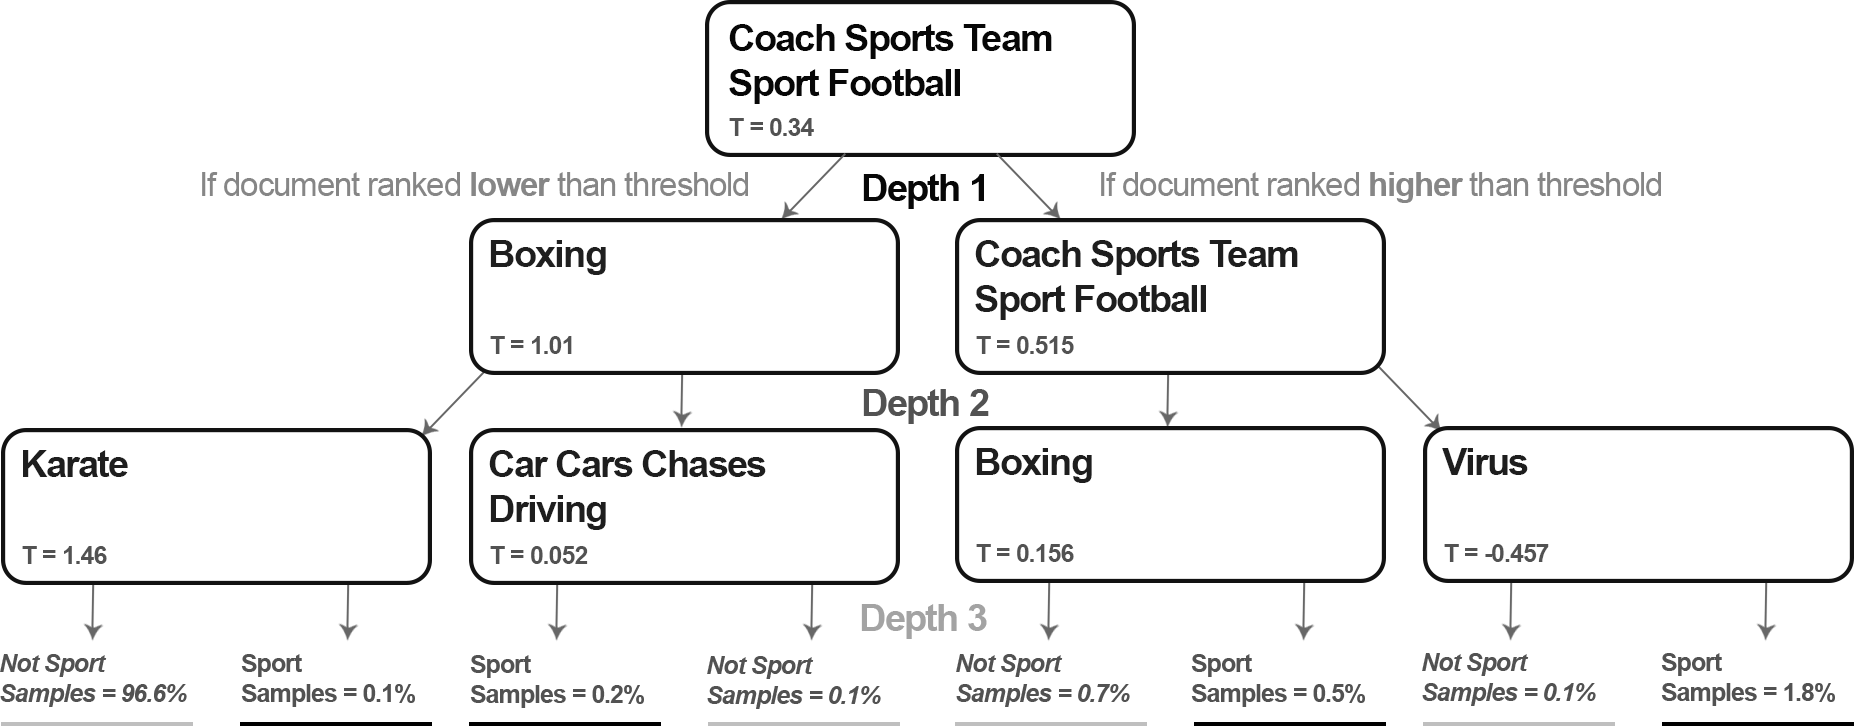
\includegraphics[width=450px]{images/decision_tree_ex.png}
	\centering
	\caption{An example of a Decision Tree classifying if a movie is in the "Sports" genre. Each Decision Tree Node corresponds to a feature, and the threshold T is the required ranking of a document on that feature to traverse right down the tree instead of left. One interesting point to note is that the most important direction is used twice, the "coach, sports, team, sport, football" cluster and results in a majority of negative samples. Another point is that the nodes at depth three are more specific, sometimes overfitting (e.g. in the case of the "Virus" node, likely overfitting to a single movie about a virus) }\label{ch3:DecisionTree}
\end{figure}




\subsection{Hyper-Parameters}\label{ch3:hyperparam}

 As stated previously (See Section \ref{ch25:reps}) in all experiments the document embedding models that results are obtained for are Doc2Vec, Principal Component Analysis (PCA), Multi-Dimensional Scaling (MDS) and Averaged Word Vectors (AWV). As possible choices for the number of dimensions, we used ${dim} (50, 100, 200)$. The Doc2Vec\footnote{Doc2Vec implemented in \href{https://radimrehurek.com/gensim/models/doc2vec.html}{gensim}} implementation from the gensim library is used. 

\subsubsection{Classifier Parameters}

There are two classifiers that are used across all experiments. CART Decision Trees\footnote{Decision Tree implemented in \href{https://scikit-learn.org/stable/modules/generated/sklearn.tree.DecisionTreeClassifier.html}{scikit-learn}} and linear SVM's \footnote{Implemented in \href{https://scikit-learn.org/stable/modules/generated/sklearn.tree.DecisionTreeClassifier.html}{scikit-learn}}.

Each SVM is also hyper-parameter tuned to find the best C values    $ C (1.0, 0.01, 0.001, 0.000)$, the best gamma value $gamma (1.0, 0.01, 0.001, 0.000)$ and if the  weights should be balanced such that positive instances are weighted in proportion to how rare they are ${balanced} (0, 1)$\footnote{Weights implemented in  \href{https://scikit-learn.org/stable/modules/generated/sklearn.utils.class_weight.compute_class_weight.html}{scikit-learn}}. In particular, where $n$ is the number of documents, and $y$ is the number of documents that are classified positively by a binary class, the weight of a class is equal to:


\begin{align}
\frac{n}{2 * y} 
\end{align}


Additionally, each Decision Tree  is hyper-parameter tuned for the following parameters:
	
\begin{itemize}
	\item The number of features\footnote{"max\_features" in scikit-learn} to consider when looking for the best split. $(none, auto, log2)$, where $none$ means that all $n$ features are considered,  $auto$ means that the maximum features considered is $\sqrt{n}$, and $log2$ which means that the number of features considered is $log2(n)$
	\item The scoring criterion for a node split $criterion: gini, entropy$. Where $gini$ is the gini impurity and $entropy$ is the information gain, see Section \ref{bg:trees} for more detail.
	\item If the  weights should be balanced ${balanced} (0, 1)$
\end{itemize} 

A parameter in the decision tree that is not tuned but is used is the maximum depth.

\subsubsection{Experiment One: Obtaining baselines}

These are three different steps of experimentation. The first experiment is to determine the best document embedding models for performance when used as input to depth-one, depth-two, depth-three and unbounded decision trees, as well as a linear SVM.  This provides a frame of reference for the later experiments for disentanglement in the case of the depth-limited trees and baseline performance on the task in the case of the linear SVM. In addition to the unsupervised document embedding models, two additional document models are included as reference: a bag-of-words of PPMI scores (BOW-PPMI) and a Latent Dirchlet Allocation (LDA) topic model. The BOW-PPMI is used as a reference for a standard performance baseline representation on the task, and the LDA topic model is used as a reference interpretable representation (where the information in the unstructured text is separated into topics). After the original filtering done to the vocabulary where either only the top 100,000 most frequent terms are used, or those that did not occur more than once are removed, the BOW-PPMI additionally has all terms filtered out that do not occur in at least $0.1\%$ of documents. This is to limit the memory requirements of the representation, but also to ensure that noisy terms that can be overfit on are not included as features.   To determine the best parameters for Doc2Vec, the following parameters are tuned: 

\begin{itemize}
	\item The ${window size} (5, 10, 15)$ referring to the context window of the words that  used   during training.
	\item The ${min count} (1, 5, 10)$ referring to the minimum frequency of words  included during training.
	\item The number of times the data is iterated on when training ${epochs} (50, 100, 200)$.
\end{itemize}

The best doc2vec embedding for each task is the one that performs best when used as input to a linear SVM. The idea is that if the representation can be separated for the key domain tasks with a linear SVM then it should contain informative directions. Additionally, the Topic Models need to be tuned. For the Latent Dirchlet Allocation topic models\footnote{Topic models implemented in \href{https://scikit-learn.org/stable/modules/generated/sklearn.decomposition.LatentDirichletAllocation.html}{scikit-learn}}, the following parameters are tuned:

\begin{itemize}
\item The prior of the document topic distribution \textit{ (0.001, 0.01, 0.1)}.
\item The prior of the topic word distribution \textit{ (0.001, 0.01, 0.1)}.
\end{itemize}


\subsubsection{Experiment Two: The best single-term property features}

The objective of this experiment is to verify that the single-term property features are disentangled. It may be the case that clustering directions does more harm to the feature representation than good, so these experiments are used to investigate the use of a feature representation composed only of rankings  entities on single terms. This is done  by using feature representations composed of single term property rankings as input to low-depth Decision Trees. This experiment also finds  the best-performing parameters on the task for the single-directions. The end-result is that for each task, there will be a best performing document embedding model and size of that model (e.g. Doc2Vec of size 50), and the following hyper-parameters are optimized for that model:

\begin{itemize}
	\item The frequency cut-off of the terms $f (20000, 10000, 5000) $, where directions are only obtained for terms in the top $f$.
	\item The score cut-off of the directions $s (2000, 1000)$, where the feature-representation used as input to the classifiers is composed of rankings of entities on the top $s$ directions.
	\item The score-type \textit{t ({F1}, {Kappa}, {Accuracy}, {NDCG})} which is the method used to score the directions.
\end{itemize}

The reason these hyper-parameters are optimized are because even the top-scoring directions are not always meaningful, as  observed in the qualitative analysis in Table \ref{ch3:scoringtypes} for example.

%Each Decision Tree has its own set of hyper-parameters that are optimized. These are the models trained on the training data and scored on the test data, with the highest performing in terms of F1-score parameters from hyper-parameter optimization on the development data. For ease of comparison, some results are provided with \dfrac{num}{den}SVM's and unbounded Decision Trees, as well as a baseline Topic Model, which is used as a reference for a standard approach to obtaining a representation where features are key aspects of the domain. Below, the parameters are listed that are optimized for each of these model types:




\subsubsection{Experiment Three: The best cluster features}

The objective of this experiment is to verify that the cluster features are disentangled. Clustering is an alternative method to using single-term directions that combines the directions into clusters. This results in a lower amount of linearly combined features labelled with clusters of words. As in the last experiment, this is done by using a feature-representation composed of cluster-rankings as input to low-depth Decision Trees.  The two different clustering methods,  K-means\footnote{K-means implemented in \href{https://scikit-learn.org/stable/modules/generated/sklearn.cluster.MiniBatchKMeans.html}{scikit-learn}} and Derrac's k-means variation (as described in Section \ref{ch3:LabellingWords}), are used. The best single-term property parameters are used as the basis of this experiment, where for each classifier and task the clusters are obtained from the top $s$ directions and score-type $t$,  chosen by hyper-parameter optimization for that classifier and task. The only hyper-parameter optimized in this experiment is the amount of clusters.





%For the clustering, the optimal directions as decided by the single direction experiments is chosen, and the same frequency and score thresholds are used as was optimally chosen. As these algorithms select centroids from the top-scoring directions or randomly, we can expect that some clusters may not be salient features of the document embedding model. This is because top-scoring directions, e.g. for accuracy could simply infrequent terms that do not have much meaning, and these infrequent terms could also be randomly selected. We could use grid-search on the frequency and score cutoffs when obtaining these results in order to avoid terms that may disrupt existing clusters or form cluster centers that are not salient features of the document embedding model, but we chose a more standardized process that would rely on the parameters of the clustering algorithms and the ability of the classifiers to filter out clusters that are not informative, so as to not make a time-costly grid search a necessary part of the process.

%The parameters that are desirable to determine are the type of document embedding model, the size of the document embedding model, the frequency threshold and the score threshold, which determines the top scoring directions. To do so, for each document embedding model of each size, a grid search is used to find the best frequency and score cut-offs for that sized document embedding model. Then, from these document embedding models and sizes the best performing one is selected. There is a balance between finding words which are useful for creating salient features in our clustering step without including too many words which do not. As our clustering methods are unsupervised, it is important that the amount of noise being entered into them is limited, despite the classifiers that use these directions typically being able to filter out those directions which are not suitable to the class. Additionally, as the vocabulary size varies from dataset to dataset, the threshold will naturally be different for each one. 

	
%\subsubsection{Representations used}

%For the baselines, four different document embedding models are used, a Bag-Of-Words of PPMI (BOW-PPMI) scores and a standard Latent Dirchlet Allocation (LDA) Topic Model.  
%The MDS document embedding model is not available for sentiment, as the memory cost was too prohibitive with 50,000 documents, and there are no doc2vec embeddings for placetypes/movies, as it was only possible access to the Bag-Of-Words representation.

%As the doc2vec has already been hyper-parameter optimized, the optimal doc2vec embedding that scored the highest for its class on a Linear SVM is used, rather than tuning the entire process around the doc2vecs vectors. So for example, when evaluating the Keywords task for the movies, directions are obtained from the doc2vec embedding that performed best for a linear SVM on the Keywords task following the previous experiments. 



\subsection{Summary of all Results}

 Table \ref{bg:repsresults} is a summary of the three experiments, listing results of different representations on trees limited to depth-one, two and three. As expected, the original entangled unsupervised document embeddings did not perform well on this task. In contrast, single-directions and clusters of these single-directions obtained from these document embedding models out-perform the bag-of-words in most cases, with two exceptions being the depth-two tree for the place-types domain and the depth-one tree on the movies keywords task. 

For the keywords task,  in a depth-1 tree, finding words that  directly correspond to particular keywords is simple with the BOW-PPMI representation. As the words that are able to classify these keywords will typically be infrequent (e.g. "new york city", "father-son relationship"), they are likely not as well-represented spatially in the  document embedding model. In this case, the PPMI representation is suitable, as it can find 1-1 matches with the classes without modelling similarity information. When using depth-two and depth-three limited decision trees, the score is no-longer as good for PPMI, which is likely  due to overfitting. 

Sometimes Decision Trees of depth-two outperform those of depth-one, but generally depth-three trees perform best.  In the case of the place-types, although topic models and PPMI representations are indeed the best, it is not by a wide-margin. Meanwhile when the single directions perform the best in these domains for other tree types they perform much better than the other approaches. Additionally, place-types has the least entities for its tasks and the tasks are very unbalanced, so it is possible that they overfit. 



\afterpage{
\begin{landscape}
	\begin{table}[]
		\small
		\centering
		\begin{tabular}{llll@{\hskip 0.25in}lll@{\hskip 0.25in}lllll}
			& Genres                          &              &               & Keywords                        &                 &                       & Ratings                         &                      &    
			                 &  & \\
			Movies            & D1                              & D2                              & D3                              & D1                              & D2                              & D3                              & D1                              & D2                              & D3                              &             &             \\
			\toprule[\heavyrulewidth]
			Space             & 0.301                           & 0.358                           & 0.354                           & 0.185                           & 0.198                           & 0.201                           & 0.463                           & 0.475                           & 0.486                           &             &             \\
			Single directions & \textbf{0.436} & 0.463                           & 0.492                           & 0.23                            & \textbf{0.233} & \textbf{0.224} & 0.466                           & 0.499                           & 0.498                           &             &             \\
			Clusters          & 0.431                           & \textbf{0.513} & \textbf{0.506} & 0.215                           & 0.22                            & 0.219                           & \textbf{0.504} & \textbf{0.507} & \textbf{0.513} &             &             \\
			PPMI              & 0.429                           & 0.443                           & 0.483                           & \textbf{0.243} & 0.224                           & 0.224                           & 0.47                            & 0.453                           & 0.453                           &             &             \\
			Topic             & 0.415                           & 0.472                           & 0.455                           & 0.189                           & 0.05                            & 0.075                           & 0.473                           & 0.243                           & 0.38                            &             &             \\
			& Newsgroups                      &                                 &                                 & Sentiment                       &                                 &                                 & Reuters                         &                                 &                                 &             &             \\

			\toprule[\heavyrulewidth]
			Rep               & 0.251                           & 0.366                           & 0.356                           & 0.705                           & 0.77                            & 0.773                           & 0.328                           & 0.413                           & 0.501                           &             &             \\
			Single dir        & 0.418                           & \textbf{0.49}  & \textbf{0.537} & 0.784                           & 0.814                           & \textbf{0.821} & \textbf{0.678} & \textbf{0.706} & 0.72                            &             &             \\
			Cluster           & 0.394                           & 0.433                           & 0.513                           & 0.735                           & \textbf{0.844} & 0.813                           & 0.456                           & 0.569                           & 0.583                           &             &             \\
			PPMI              & 0.33                            & 0.407                           & 0.444                           & 0.7                             & 0.719                           & 0.73                            & 0.616                           & 0.699                           & \textbf{0.723} &             &             \\
			Topic             & \textbf{0.431} & 0.423                           & 0.444                           & \textbf{0.79}  & 0.791                           & 0.811                           & 0.411                           & 0.527                           & 0.536                           &             &             \\
			& Foursquare                      &                                 &                                 & OpenCYC                         &                                 &                                 & Geonames                        &                                 &                                 &             &             \\
			Placetypes        & D1                              & D2                              & D3                              & D1                              & D2                              & D3                              & D1                              & D2                              & D3                              &             &             \\
			\toprule[\heavyrulewidth]
			Rep               & 0.438                           & 0.478                           & 0.454                           & 0.383                           & 0.397                           & 0.396                           & 0.349                           & 0.34                            & 0.367                           &             &             \\
			Single dir        & \textbf{0.541} & 0.498                           & \textbf{0.531} & 0.404                           & \textbf{0.428} & 0.39                            & \textbf{0.444} & \textbf{0.533} & \textbf{0.473} &             &             \\
			Cluster           & 0.462                           & 0.507                           & 0.496                           & \textbf{0.413} & 0.42                            & \textbf{0.429} & 0.444                           & 0.458                           & 0.47                            &             &             \\
			PPMI              & 0.473                           & \textbf{0.512} & 0.491                           & 0.371                           & 0.351                           & 0.352                           & 0.361                           & 0.301                           & 0.242                           &             &             \\
			Topic             & 0.488                           & 0.433                           & 0.526                           & 0.365                           & 0.271                           & 0.313                           & 0.365                           & 0.3                             & 0.219                           &             &             \\   
		\end{tabular}
		\caption{The F1-scores of trees limited to depth-one, two and three, for the best hyper-parameter variation of each representation}
	\end{table}\label{bg:repsresults}
\end{landscape}
}
\subsection{Baseline Representations}

In Table \ref{ch3:represults} Decision Trees and SVM results are shown when the document embeddings, the baseline representation BOW-PPMI, and the topic model features are used as input. In the case of the topic model and doc2vec, these representations are tuned. These representations serve as a reference point for what is possible using standard linear models, as well as a measure of the disentanglement of the original unsupervised document embeddings. The unsupervised document embeddings when used as input representations to depth three trees perform significantly worse in depth one trees. This is expected given the fact that these representations are entangled, so it is unlikely that a smaller tree can use the available dimensions to model a class. There are two tables, Table \ref{ch3:represults} that covers the results for the newsgroups in full detail (including more parameters, and the precision and recall scores), and Table \ref{ch3:represults_all} that shows results for all other domains but only shows the best document embeddings out of the different sizes.  Note that in Table \ref{ch3:represults} some recall scores are very high.  Recall scores are higher when the weights are balanced, as favouring  positive instances results in more positives being identified correctly. 


As seen in  Table \ref{ch3:represults}, the biggest differences in F1-score occur when the document embedding model changes, rather than when the size of document embedding model changes. For this reason, and to reserve space, only the best performing representation of each type are shown in Table \ref{ch3:represults}.  

In  Table \ref{ch3:represults} for the newsgroups, the linear SVM only achieved strong performance when using   doc2vec or PCA as input, and in the  unbounded depth decision tree PCA performed far better than the other unsupervised document embeddings. Similarly for reuters and sentiment, the PCA representation performs better than the other unsupervised document embeddings. This suggests that the linear combinations used in the PCA representation result in a more linearly separable space. The performance gap only widens when looking at low-depth decision trees that use the PCA dimensions as input, which suggests that the individual dimensions of the other unsupervised embeddings are less informative than those of the PCA spaces. This is likely due to the fact that PCA  PCA tries to select the most informative dimensions, whereas the dimensions of the other representations are more or less arbitrary. However, this does not tell us anything about the quality of the directions that can be learned in both types of spaces. 

In the single directions results, PCA is outperformed by MDS and other representations in F1 score for low Decision Tree depths in any of these domains, with the exception of the depth-two trees for sentiment. Despite MDS not having informative dimensions, our method is still able to obtain a distangled feature representation from this document embedding. There is a low correlation  between performance on the raw dimensions of the space and performance with rankings on directions in low-depth Decision Trees.  Despite the information encoded in the space, if it is not disentangled then the classifier will not perform well.


\afterpage{
\begin{landscape}
\begin{table}[]
	\scriptsize
	\begin{tabular}{lllll@{\hskip 0.25in}llll@{\hskip 0.25in}llll@{\hskip 0.25in}llll@{\hskip 0.25in}lllll}
		Newsgroups & D1                              &                                 &                                 &                                 & D2                              &                                 &                                 &                                 & D3                              &                                 &                                 &                                 & DN                              &                                 &                                 &                                 & SVM                             &                                 &                                 &                                 &                                 \\
& ACC                             & F1                              & Prec                            & Rec                             & ACC                             & F1                              & Prec                            & Rec                             & ACC                             & F1                              & Prec                            & Rec                             & ACC                             & F1                              & Prec                            & Rec                             & ACC                             & F1                              & Prec                            & Rec                             &                                 \\
\toprule[\heavyrulewidth]
PCA 200    & 0.701                           & 0.251                           & 0.148                           & 0.811                           & 0.843                           & 0.366                           & 0.245                           & 0.719                           & 0.956                           & 0.355                           & 0.54                            & 0.265                           & 0.946                           & 0.44                            & 0.45                            & 0.432                           & 0.969                           & 0.612                           & 0.746                           & 0.519                           &                                 \\
PCA 100    & 0.698                           & 0.247                           & 0.146                           & 0.813                           & 0.835                           & 0.362                           & 0.241                           & 0.731                           & 0.957                           & 0.356                           & 0.576                           & 0.257                           & 0.948                           & 0.451                           & 0.465                           & 0.438                           & 0.969                           & 0.586                           & 0.768                           & 0.474                           &                                 \\
PCA 50     & 0.68                            & 0.24                            & 0.141                           & 0.829                           & 0.834                           & 0.355                           & 0.234                           & 0.735                           & 0.957                           & 0.329                           & 0.472                           & 0.253                           & 0.947                           & 0.45                            & 0.462                           & 0.438                           & 0.966                           & 0.52                            & 0.745                           & 0.399                           &                                 \\
\midrule[\heavyrulewidth]
AWV 200    & 0.687                           & 0.217                           & 0.126                           & 0.781                           & 0.758                           & 0.256                           & 0.156                           & 0.718                           & 0.764                           & 0.26                            & 0.157                           & 0.751                           & 0.937                           & 0.339                           & 0.352                           & 0.328                           & 0.961                           & 0.468                           & 0.641                           & 0.369                           &                                 \\
AWV 100    & 0.677                           & 0.21                            & 0.122                           & 0.775                           & 0.78                            & 0.275                           & 0.173                           & 0.683                           & 0.746                           & 0.25                            & 0.149                           & 0.769                           & 0.934                           & 0.324                           & 0.332                           & 0.317                           & 0.865                           & 0.4                             & 0.265                           & 0.812                           &                                 \\
AWV 50     & 0.696                           & 0.219                           & 0.127                           & 0.772                           & 0.777                           & 0.272                           & 0.168                           & 0.71                            & 0.743                           & 0.25                            & 0.149                           & 0.786                           & 0.935                           & 0.325                           & 0.335                           & 0.316                           & 0.842                           & 0.362                           & 0.233                           & 0.819                           &                                 \\
\midrule[\heavyrulewidth]
MDS 200    & 0.581                           & 0.184                           & 0.103                           & \textbf{0.837} & 0.742                           & 0.262                           & 0.16                            & 0.729                           & 0.719                           & 0.236                           & 0.139                           & 0.785                           & 0.935                           & 0.327                           & 0.332                           & 0.323                           & 0.965                           & 0.501                           & \textbf{0.802} & 0.364                           &                                 \\
MDS 100    & 0.586                           & 0.187                           & 0.105                           & 0.833                           & 0.754                           & 0.261                           & 0.159                           & 0.727                           & 0.705                           & 0.236                           & 0.138                           & \textbf{0.808} & 0.935                           & 0.33                            & 0.338                           & 0.321                           & 0.878                           & 0.439                           & 0.308                           & 0.765                           &                                 \\
MDS 50     & 0.593                           & 0.153                           & 0.087                           & 0.647                           & 0.716                           & 0.25                            & 0.15                            & \textbf{0.756} & 0.736                           & 0.243                           & 0.144                           & 0.774                           & 0.935                           & 0.324                           & 0.335                           & 0.313                           & 0.854                           & 0.394                           & 0.259                           & 0.821                           &                                 \\
\midrule[\heavyrulewidth]
D2V 200    & 0.682                           & 0.205                           & 0.119                           & 0.746                           & 0.802                           & 0.268                           & 0.169                           & 0.646                           & 0.77                            & 0.269                           & 0.164                           & 0.75                            & 0.94                            & 0.366                           & 0.389                           & 0.346                           & 0.961                           & 0.468                           & 0.641                           & 0.369                           &                                 \\
D2V 100    & 0.682                           & 0.208                           & 0.12                            & 0.762                           & 0.792                           & 0.268                           & 0.168                           & 0.662                           & 0.786                           & 0.268                           & 0.164                           & 0.727                           & 0.94                            & 0.376                           & 0.392                           & 0.361                           & \textbf{0.971} & \textbf{0.628} & 0.761                           & 0.535                           &                                 \\
D2V 50     & 0.683                           & 0.207                           & 0.12                            & 0.764                           & 0.809                           & 0.294                           & 0.187                           & 0.694                           & 0.782                           & 0.28                            & 0.172                           & 0.761                           & 0.943                           & 0.394                           & 0.415                           & 0.376                           & 0.97                            & 0.601                           & 0.758                           & 0.497                           &                                 \\
\midrule[\heavyrulewidth]
PPMI       & \textbf{0.948} & 0.33                            & \textbf{0.532} & 0.239                           & 0.947                           & 0.407                           & 0.511                           & 0.338                           & 0.944                           & \textbf{0.444} & 0.506                           & 0.396                           & \textbf{0.951} & \textbf{0.494} & \textbf{0.496} & \textbf{0.492} & 0.962                           & 0.613                           & 0.627                           & 0.599                           &                                 \\
\midrule[\heavyrulewidth]
Topic      & 0.852                           & \textbf{0.431} & 0.304                           & 0.743                           & \textbf{0.96}  & \textbf{0.423} & \textbf{0.604} & 0.326                           & \textbf{0.961} & 0.444                           & \textbf{0.606} & 0.35                            & 0.944                           & 0.432                           & 0.434                           & 0.429                           & 0.879                           & 0.46                            & 0.318                           & \textbf{0.835} &                                 \\
	\end{tabular}
\caption{Best results for the newsgroups for a variety of classifiers when using the document embeddings as input.}\label{ch3:represults}
\end{table}
\end{landscape}
}


\afterpage{
\begin{landscape}
\begin{table}
	\centering
	\scriptsize
	\begin{tabular}{ll@{\hskip 0.15in}l@{\hskip 0.2in}l@{\hskip 0.15in}l@{\hskip 0.2in}l@{\hskip 0.15in}l@{\hskip 0.2in}l@{\hskip 0.15in}l@{\hskip 0.2in}l@{\hskip 0.15in}l@{\hskip 0.1in}lll@{\hskip 0.15in}l@{\hskip 0.2in}l@{\hskip 0.15in}l@{\hskip 0.2in}l@{\hskip 0.15in}l@{\hskip 0.2in}l@{\hskip 0.15in}l@{\hskip 0.2in}l@{\hskip 0.15in}l@{\hskip 0.2in}l@{\hskip 0.15in}l@{\hskip 0.2in}lll}
		Reuters    & D1              &                 & D2              &                 & D3              &                 & DN              &                 & SVM             &                 &  & Sentiment & D1              &                 & D2              &                 & D3              &                 & DN              &                 & SVM             &                  \\
		& ACC             & F1              & ACC             & F1              & ACC             & F1              & ACC             & F1              & ACC             & F1              &  &           & ACC             & F1              & ACC             & F1              & ACC             & F1              & ACC             & F1              & ACC             & F1               \\ 

\cmidrule[\heavyrulewidth]{1-11}\cmidrule[\heavyrulewidth]{13-23}
		PCA        & 0.847           & 0.328           & 0.917           & 0.413           & 0.978           & 0.501           & 0.978           & 0.565           & 0.989           & 0.761           &  & PCA       & 0.745           & 0.705           & 0.755           & 0.77            & 0.778           & 0.773           & \textbf{0.781}  & \textbf{0.779}  & \textbf{0.891}  & \textbf{0.893}   \\
		AWV        & 0.782           & 0.252           & 0.971           & 0.328           & 0.974           & 0.417           & 0.973           & 0.495           & 0.987           & 0.719           &  & AWV       & 0.642           & 0.652           & 0.643           & 0.694           & 0.695           & 0.717           & 0.66            & 0.663           & 0.827           & 0.829            \\
		MDS        & 0.791           & 0.263           & 0.9             & 0.357           & 0.979           & 0.489           & 0.976           & 0.522           & 0.988           & 0.67            &  & D2V       & 0.642           & 0.664           & 0.66            & 0.707           & 0.702           & 0.7             & 0.711           & 0.708           & 0.878           & 0.878            \\
		D2V        & 0.818           & 0.268           & 0.867           & 0.298           & 0.974           & 0.445           & 0.971           & 0.482           & 0.986           & 0.724           &  & PPMI      & 0.616           & 0.7             & 0.655           & 0.719           & 0.675           & 0.73            & 0.712           & 0.71            & 0.887           & 0.888            \\
		PPMI       & \textbf{0.975}  & \textbf{0.616}  & \textbf{0.978}  & \textbf{0.699}  & \textbf{0.98}   & \textbf{0.723}  & \textbf{0.984}  & \textbf{0.746}  & \textbf{0.99}   & \textbf{0.8}    &  & Topic     & \textbf{0.793}  & \textbf{0.79}   & \textbf{0.794}  & \textbf{0.791}  & \textbf{0.81}   & \textbf{0.811}  & 0.733           & 0.73            & 0.815           & 0.822            \\
		Topic      & 0.92            & 0.411           & 0.977           & 0.527           & 0.977           & 0.536           & 0.977           & 0.56            & 0.95            & 0.513           &  &           &                 &                 &                 &                 &                 &                 &                 &                 &                 &                  \\
		&                 &                 &                 &                 &                 &                 &                 &                 &                 &                 &  &           &                 &                 &                 &                 &                 &                 &                 &                 &                 &                  \\
		Placetypes & D1              &                 & D2              &                 & D3              &                 & DN              &                 & SVM             &                 &  & Movies    & D1              &                 & D2              &                 & D3              &                 & DN              &                 & SVM             &                  \\
		OpenCYC    & ACC             & F1              & ACC             & F1              & ACC             & F1              & ACC             & F1              & ACC             & F1              &  & Genres    & ACC             & F1              & ACC             & F1              & ACC             & F1              & ACC             & F1              & ACC             & F1               \\ 
		\cmidrule[\heavyrulewidth]{1-11}\cmidrule[\heavyrulewidth]{13-23}
		PCA        & 0.586           & 0.346           & 0.708           & 0.343           & 0.695           & 0.342           & 0.832           & 0.309           & 0.847           & 0.474           &  & PCA       & 0.722           & 0.301           & 0.755           & 0.339           & 0.717           & 0.321           & 0.884           & 0.372           & \textbf{0.925}  & 0.518            \\
		AWV        & 0.625           & \textbf{0.383}  & 0.651           & 0.376           & 0.728           & \textbf{0.396}  & \textbf{0.844}  & \textbf{0.362}  & 0.85            & 0.466           &  & AWV       & 0.679           & 0.29            & 0.774           & 0.321           & 0.756           & 0.343           & 0.873           & 0.312           & 0.922           & 0.496            \\
		MDS        & 0.624           & 0.364           & 0.7             & \textbf{0.397}  & 0.731           & 0.374           & 0.843           & 0.305           & 0.861           & \textbf{0.476}  &  & MDS       & 0.679           & 0.298           & 0.79            & 0.358           & 0.773           & 0.354           & 0.887           & 0.385           & 0.875           & \textbf{0.532}   \\
		PPMI       & \textbf{0.728}  & 0.371           & 0.75            & 0.351           & 0.739           & 0.352           & 0.843           & 0.323           & \textbf{0.9}    & 0.366           &  & PPMI      & \textbf{0.852}  & \textbf{0.429}  & \textbf{0.91}   & 0.443           & \textbf{0.912}  & \textbf{0.483}  & 0.882           & \textbf{0.416}  & 0.923           & 0.526            \\
		Topic      & 0.708           & 0.365           & \textbf{0.87}   & 0.271           & \textbf{0.87}   & 0.313           & 0.831           & 0.313           & 0.808           & 0.407           &  & Topic     & 0.767           & 0.415           & 0.905           & \textbf{0.472}  & 0.912           & 0.455           & \textbf{0.889}  & 0.415           & 0.843           & 0.491            \\
		&                 &                 &                 &                 &                 &                 &                 &                 &                 &                 &  &           &                 &                 &                 &                 &                 &                 &                 &                 &                 &                  \\
		Placetypes & D1              &                 & D2              &                 & D3              &                 & DN              &                 & SVM             &                 &  & Movies    & D1              &                 & D2              &                 & D3              &                 & DN              &                 & SVM             &                  \\
		Foursquare & ACC             & F1              & ACC             & F1              & ACC             & F1              & ACC             & F1              & ACC             & F1              &  & Keywords  & ACC             & F1              & ACC             & F1              & ACC             & F1              & ACC             & F1              & ACC             & F1               \\ 
		\cmidrule[\heavyrulewidth]{1-11}\cmidrule[\heavyrulewidth]{13-23}
		PCA        & 0.731           & 0.342           & 0.823           & 0.393           & 0.86            & 0.388           & 0.887           & 0.398           & 0.896           & 0.568           &  & PCA       & 0.647           & 0.185           & 0.644           & 0.193           & 0.677           & 0.199           & 0.846           & 0.161           & 0.787           & 0.272            \\
		AWV        & 0.767           & 0.401           & 0.828           & 0.478           & 0.85            & 0.452           & 0.905           & \textbf{0.505}  & 0.923           & \textbf{0.622}  &  & AWV       & 0.5             & 0.16            & 0.641           & 0.179           & 0.595           & 0.174           & 0.853           & 0.141           & 0.717           & 0.23             \\
		MDS        & \textbf{0.915}  & 0.438           & 0.804           & 0.427           & 0.86            & 0.454           & 0.893           & 0.462           & 0.932           & 0.619           &  & MDS       & 0.633           & 0.179           & 0.69            & 0.198           & 0.674           & 0.201           & 0.84            & 0.163           & 0.788           & \textbf{0.28}    \\
		PPMI       & 0.889           & 0.473           & 0.915           & \textbf{0.512}  & 0.904           & 0.491           & 0.881           & 0.31            & \textbf{0.938}  & 0.567           &  & PPMI      & \textbf{0.818}  & \textbf{0.243}  & 0.745           & \textbf{0.224}  & 0.739           & \textbf{0.224}  & 0.847           & \textbf{0.17}   & \textbf{0.921}  & 0.217            \\
		Topic      & 0.864           & \textbf{0.488}  & \textbf{0.916}  & 0.433           & \textbf{0.917}  & \textbf{0.526}  & \textbf{0.907}  & 0.464           & 0.916           & 0.569           &  & Topic     & 0.629           & 0.189           & \textbf{0.932}  & 0.05            & \textbf{0.93}   & 0.075           & \textbf{0.857}  & 0.152           & 0.678           & 0.21             \\
		&                 &                 &                 &                 &                 &                 &                 &                 &                 &                 &  &           &                 &                 &                 &                 &                 &                 &                 &                 &                 &                  \\
		Placetypes & D1              &                 & D2              &                 & D3              &                 & DN              &                 & SVM             &                 &  & Movies    & D1              &                 & D2              &                 & D3              &                 & DN              &                 & SVM             &                  \\
		Geonames   & ACC             & F1              & ACC             & F1              & ACC             & F1              & ACC             & F1              & ACC             & F1              &  & Ratings   & ACC             & F1              & ACC             & F1              & ACC             & F1              & ACC             & F1              & ACC             & F1               \\ 
		\cmidrule[\heavyrulewidth]{1-11}\cmidrule[\heavyrulewidth]{13-23}
		PCA        & 0.502           & 0.301           & 0.69            & 0.305           & 0.68            & 0.295           & 0.821           & 0.243           & 0.844           & 0.401           &  & PCA       & \textbf{0.65}   & 0.463           & 0.681           & \textbf{0.475}  & 0.684           & \textbf{0.486}  & 0.744           & 0.408           & 0.771           & 0.58             \\
		AWV        & 0.657           & 0.326           & 0.755           & 0.323           & 0.842           & \textbf{0.367}  & 0.813           & 0.332           & 0.865           & \textbf{0.514}  &  & AWV       & 0.601           & 0.423           & 0.618           & 0.433           & 0.596           & 0.448           & 0.736           & 0.372           & 0.73            & 0.532            \\
		MDS        & 0.626           & 0.349           & 0.695           & \textbf{0.34}   & 0.796           & 0.272           & \textbf{0.845}  & 0.295           & 0.638           & 0.397           &  & MDS       & 0.592           & 0.437           & 0.635           & 0.449           & 0.631           & 0.452           & \textbf{0.752}  & \textbf{0.412}  & 0.773           & \textbf{0.589}   \\
		PPMI       & \textbf{0.808}  & 0.361           & 0.732           & 0.301           & 0.76            & 0.242           & 0.83            & 0.283           & \textbf{0.894}  & 0.312           &  & PPMI      & 0.583           & 0.47            & 0.635           & 0.453           & 0.605           & 0.453           & 0.73            & 0.384           & \textbf{0.825}  & 0.536            \\
		Topic      & 0.771           & \textbf{0.365}  & \textbf{0.863}  & 0.3             & \textbf{0.85}   & 0.219           & 0.828           & \textbf{0.348}  & 0.819           & 0.349           &  & Topic     & 0.575           & \textbf{0.473}  & \textbf{0.789}  & 0.243           & \textbf{0.789}  & 0.38            & 0.739           & 0.375           & 0.704           & 0.501           
	\end{tabular}\caption{Best results for all domains for a variety of classifiers when using the document embeddings as input.}\label{ch3:represults_all}
\end{table}
\end{landscape}
}




\subsection{Word Directions}

In Table \ref{ch3:singledirs} the results for the feature representation composed of rankings of entities on single-term directions that performed best when used as input to a classifier is shown.

%Although Linear SVM's perform the best on these representations, other results will be for low-depth Decision Trees in-order to easily distinguish how well  key semantics are disentangled  in the representations.


 
 As can be seen for the newsgroups results in Table \ref{ch3:singledirs}, the number of dimensions now has a bigger impact on the results, in particular for the depth-three and two trees. This difference was smaller for the depth-one trees. This is likely because despite the size of the document embedding model, they all modelled a similar most-important single direction relevant to the task, e.g. a direction that can classify if the entity is religious like the word-direction for "celestial". However, variants of the space size change the representation of auxiliary directions that are not as relevant to the task but are useful when the depth is higher for the tree.
 
 
The best space type also varied across domains, e.g. the classifiers performed best for reuters with a disentangled single-term feature representation obtained from MDS used as input, but a feature representation obtained from Doc2Vec when used as input performed best for newsgroups. Loosely, it is possible to attribute the performance increase for a space-type to an increased score (e.g. NDCG score) for relevant directions to the class. When looking at the qualitative results, generally the words common to all space-types are the most salient, as can be seen in Table \ref{ch3:ComparingSpaceTypes}, so in this case the increased results for different hyper-parameters likely comes down to either these common directions being better modelled in the representation or terms that were not modelled well before that were relevant to the task being modelled better.
 
 %We can see if this is the case by looking at the Decision Trees for the same task that had the most difference between the space-types and space-sizes. If a Decision Tree contains mostly similar words, but the performance is greater, we can attribute it to a better quality ranking in the space. If the Decision Tree contains different words, especially as the first node, then we know that it was because the words that were modelled well were different between them. 
 
 We see that generally, the best document embedding model is the same across the same domain: specifically AWV is the best for the place-types but MDS is best for the movies (despite a marginal difference in the ratings). Generally, this  means that these document embedding types in particular are good at modelling informative properties for the tasks. 
 
 Although some tasks on some classifiers did perform better using score-types like F1-score, in general, filtering directions by NDCG score performed the best. In particular it was found  the best score-type for Sentiment, Newsgroups, Reuters, Movies Genres, Movies Keywords in depth-3 Decision Trees.  In conclusion, the document embedding model is an important hyper-parameter to tune for each domain, as is the size of that document embedding. However, document embeddings that perform well on one task may be good at the others too. Finally, NDCG is a good scoring metric to use for finding features that are meaningful in the representation.
 

 %To investigate why space-types perform better than others for each domain, we compare the Decision Trees where there is the most difference. For the genres, MDS outperforms PCA and AWV on the genres task by 0.03. 

%What is the importance of the space size?
%What is the importance of the space type?
%How do directions perform compared to spaces? Why?
%What kind of directions do we find for each score type?
%Why does the score type matter? What score type works best?

%These single directions typically overfit.
\afterpage{
\begin{landscape}
\begin{table}[]
	\centering
	\scriptsize
	\begin{tabular}{llllllllllllll}
Newsgroups & D1                              &                  &                &                       & D2                              &                     &                    &      & D3                              &                &                &         &                    \\
& ACC                             & F1                              & Prec                            & Rec                             & ACC                             & F1                              & Prec                            & Rec                             & ACC                             & F1                              & Prec                            & Rec                             &                                 \\
PCA 200    & 0.955                           & 0.348                           & 0.521                           & 0.261                           & 0.959                           & 0.424                           & 0.678                           & 0.309                           & 0.96                            & 0.454                           & 0.674                           & 0.343                           &                                 \\
PCA 100    & 0.957                           & 0.382                           & 0.491                           & 0.313                           & 0.961                           & 0.474                           & 0.679                           & 0.364                           & \textbf{0.963} & 0.512                           & 0.694                           & 0.406                           &                                 \\
PCA 50     & 0.957                           & 0.373                           & 0.417                           & 0.337                           & \textbf{0.963} & 0.478                           & 0.621                           & 0.388                           & 0.963                           & 0.506                           & 0.7                             & 0.396                           &                                 \\
AWV 200    & 0.832                           & 0.35                            & 0.226                           & 0.777                           & 0.957                           & 0.383                           & 0.517                           & 0.305                           & 0.958                           & 0.445                           & 0.598                           & 0.354                           &                                 \\
AWV 100    & 0.83                            & 0.343                           & 0.219                           & 0.785                           & 0.823                           & 0.36                            & 0.233                           & \textbf{0.792} & 0.956                           & 0.387                           & 0.563                           & 0.295                           &                                 \\
AWV 50     & 0.807                           & 0.341                           & 0.215                           & 0.816                           & 0.833                           & 0.361                           & 0.236                           & 0.762                           & 0.954                           & 0.392                           & 0.511                           & 0.318                           &                                 \\
MDS 200    & \textbf{0.959} & \textbf{0.418} & \textbf{0.543} & 0.339                           & 0.962                           & 0.465                           & 0.669                           & 0.357                           & 0.962                           & 0.493                           & \textbf{0.707} & 0.379                           &                                 \\
MDS 100    & 0.857                           & 0.365                           & 0.244                           & 0.725                           & 0.959                           & 0.428                           & 0.624                           & 0.326                           & 0.96                            & 0.453                           & 0.644                           & 0.349                           &                                 \\
MDS 50     & 0.821                           & 0.324                           & 0.206                           & 0.762                           & 0.842                           & 0.386                           & 0.258                           & 0.77                            & 0.957                           & 0.398                           & 0.596                           & 0.299                           &                                 \\
D2V 200    & 0.831                           & 0.343                           & 0.22                            & 0.784                           & 0.96                            & 0.47                            & \textbf{0.683} & 0.358                           & 0.962                           & 0.494                           & 0.69                            & 0.385                           &                                 \\
D2V 100    & 0.844                           & 0.374                           & 0.243                           & 0.803                           & 0.961                           & \textbf{0.49}  & 0.642                           & 0.396                           & 0.962                           & 0.517                           & 0.67                            & 0.421                           &                                 \\
D2V 50     & 0.845                           & 0.388                           & 0.252                           & \textbf{0.844} & 0.962                           & 0.488                           & 0.639                           & 0.395                           & 0.963                           & \textbf{0.537} & 0.673                           & \textbf{0.446} &                                 \\
&                                 &                                 &                                 &                                 &                                 &                                 &                                 &                                 &                                 &                                 &                                 &                                 &                                 \\
Reuters    & D1                              &                                 & D2                              &                                 & D3                              &                                 & Sentiment                       & D1                              &                                 & D2                              &                                 & D3                              &                                 \\
& ACC                             & F1                              & ACC                             & F1                              & ACC                             & F1                              &                                 & ACC                             & F1                              & ACC                             & F1                              & ACC                             & F1                              \\
PCA        & 0.976                           & 0.658                           & 0.979                           & 0.679                           & 0.977                           & 0.467                           & PCA                             & 0.739                           & 0.759                           & \textbf{0.797} & \textbf{0.814} & 0.802                           & 0.805                           \\
AWV        & 0.975                           & 0.598                           & 0.979                           & 0.656                           & 0.98                            & 0.66                            & AWV                             & 0.7                             & 0.699                           & 0.711                           & 0.736                           & 0.723                           & 0.735                           \\
MDS        & 0.975                           & \textbf{0.678} & \textbf{0.98}  & \textbf{0.706} & \textbf{0.982} & \textbf{0.72}  & D2V                             & \textbf{0.776} & \textbf{0.784} & 0.782                           & 0.801                           & \textbf{0.822} & \textbf{0.821} \\
D2V        & \textbf{0.977} & 0.583                           & 0.979                           & 0.664                           & 0.98                            & 0.632                           &                                 &                                 &                                 &                                 &                                 &                                 &                                 \\
Placetypes & D1                              &                                 & D2                              &                                 & D3                              &                                 & Movies                          & D1                              &                                 & D2                              &                                 & D3                              &                                 \\
OpenCYC    & ACC                             & F1                              & ACC                             & F1                              & ACC                             & F1                              & Genres                          & ACC                             & F1                              & ACC                             & F1                              & ACC                             & F1                              \\
PCA        & 0.632                           & 0.371                           & 0.704                           & 0.381                           & 0.735                           & 0.365                           & PCA                             & 0.824                           & 0.412                           & 0.82                            & 0.441                           & 0.913                           & 0.463                           \\
AWV        & \textbf{0.66}  & \textbf{0.404} & \textbf{0.734} & \textbf{0.428} & \textbf{0.755} & \textbf{0.39}  & AWV                             & 0.81                            & 0.421                           & 0.837                           & 0.436                           & 0.912                           & 0.457                           \\
MDS        & 0.658                           & 0.374                           & 0.711                           & 0.385                           & 0.746                           & 0.35                            & MDS                             & \textbf{0.849} & \textbf{0.446} & \textbf{0.839} & \textbf{0.463} & \textbf{0.918} & \textbf{0.495} \\
Foursquare & ACC                             & F1                              & ACC                             & F1                              & ACC                             & F1                              & Keywords                        & ACC                             & F1                              & ACC                             & F1                              & ACC                             & F1                              \\
PCA        & 0.785                           & 0.477                           & \textbf{0.907} & 0.474                           & 0.869                           & \textbf{0.531} & PCA                             & 0.737                           & 0.225                           & 0.727                           & 0.227                           & \textbf{0.709} & 0.22                            \\
AWV        & \textbf{0.918} & \textbf{0.541} & 0.881                           & \textbf{0.498} & 0.889                           & 0.466                           & AWV                             & 0.656                           & 0.201                           & 0.672                           & 0.203                           & 0.652                           & 0.2                             \\
MDS        & 0.82                            & 0.416                           & 0.879                           & 0.482                           & \textbf{0.897} & 0.485                           & MDS                             & \textbf{0.745} & \textbf{0.23}  & \textbf{0.74}  & \textbf{0.233} & 0.708                           & \textbf{0.224} \\
Geonames   & ACC                             & F1                              & ACC                             & F1                              & ACC                             & F1                              & Ratings                         & ACC                             & F1                              & ACC                             & F1                              & ACC                             & F1                              \\
PCA        & 0.665                           & 0.348                           & 0.754                           & 0.342                           & 0.743                           & 0.306                           & PCA                             & \textbf{0.647} & \textbf{0.466} & \textbf{0.721} & \textbf{0.499} & 0.681                           & 0.492                           \\
AWV        & \textbf{0.711} & \textbf{0.444} & \textbf{0.795} & \textbf{0.533} & \textbf{0.802} & \textbf{0.473} & AWV                             & 0.646                           & 0.463                           & 0.692                           & 0.474                           & 0.677                           & 0.483                           \\
MDS        & 0.591                           & 0.289                           & 0.772                           & 0.333                           & 0.764                           & 0.352                           & MDS                             & 0.62                            & 0.463                           & 0.692                           & 0.489                           & \textbf{0.686} & \textbf{0.498}
	\end{tabular}\label{ch3:singledirs}
	\caption{The best results (hyper-parameter tuned) for the classifiers for each task when the disentangled feature representations composed of rankings of entities on single-term directions.}
\end{table}
\end{landscape}
}

\subsection{Clustered Directions}
\ref{ch3:clusterexample}

Clustering has two main goals: The first is that features that  align with properties of entities in the domain are obtained by combining together single-word directions that reference phenomena, e.g. in a domain of movie reviews "Blood", "Scary",  "Horror" can be clustered to obtain a cluster that better models the idea of horror in film, rather than modelling individual things that occur in film. The second is that it makes the features more interpretable by providing context to the words. In this section, we examine how these more abstract and complex cluster features perform quantitatively at key domain tasks.

K-means mostly outperforms Derrac. It does not in the case of Keywords, where Derrac performs better for every Decision Tree. Although the differences in absolute values are quite small in this case, it is still significant as it is quite difficult to achieve high performance on this task, making these relative changes important. This case can give us insight into how disentanglement affects performance on different classes and domains - and how our unsupervised method selects the best parameters.  Specifically, when looking into the how the individual classes fared, when using 100 clusters, the Derrac variant clusters performed better at the keywords "shot-in-the-chest" and "machine-gun" and sacrificed performance in the "sequel" class. In Derrac, there was the following cluster ("soldiers combat fighting military battle ... weapons rambo gunfights spaghetti guns ...") while for the results of the k-means clustering method when restricted to 200 clusters these words were split into two separate clusters, one for guns ("gun explosions shoot shooting weapons ... rambo") and one for military ("war soldiers combat military ... platoon infantry"). It is possible that as the Derrac method combined these together into a single cluster it was able to better capture the classes for "shot-in-the-chest" and "machine-guns" as these keywords refer to war films where people were shot or shooting. So in this case, the clusters chosen by the  Derrac variant supported the classification of the documents. 

This idea is supported when looking at the depth-three tree for this class, which uses this cluster as its first node as well as a node in the depth-two layer. This is an instance where averaging the direction of  a heavily populated cluster  performs better than obtaining features that are more dense and less disentangled. 


%%%%%%%%%%%%

% ADD DECISION TREE

%%%%%%%%%%%

Meanwhile, this same lack of separation caused the clusters to lose performance in the "sequel" class. With the K-means method, the cluster was found for ("franchise sequels sequel installments") with the Derrac variant, the corresponding cluster was ("franchise sequels sequel instalments entry returns"). This cluster was also chosen for the Derrac variant as the first node of its Decision Tree, but this caused it to perform worse than k-means. This is likely because although the words "entry" and "returns" were most similar to this cluster, they disrupted the direction too much. Indeed, when looking at the k-means clusters, the "returns" direction is clustered with "events situation conclusion spoiler ... protagonists exscapes break scenario ...", seemingly referring to a character or thing "returning" in a conclusive part of the movie, and the word "entry" is clustered with the words "effective genuine ... hits build surprisingly ... succeeds essentially finale entry ..." seemingly relating to a more sentiment related cluster about how a movie performed. So in this case k-means found more disentangled clusters than Derrac gave it a performance advantage. 


%%%%%%%%%%%%

% ADD DECISION TREE

%%%%%%%%%%%

This could be due to the best-performing variants of the Derrac clustering method obtaining 100 clusters (meaning the clusters would contain more terms) and the best performing variants of the k-means obtaining 200 clusters. However, in the 100-size k-means clusters, "gun" and "explosions" ended up being in a cluster with ("western outlaw heist shootout west"), making it a more western oriented cluster, and the idea of a war was even more separated with a single cluster corresponding to ("war soldiers military solider army sergeant sgt platoon infantry"). In conclusion, Derrac for the Keywords task captured certain properties better than k-means, in particular by clustering together the idea of "war" and "guns" to achieve high performance on the keywords "shot-in-the-chest" and "machine-guns". k-means favoured a more separated approach to these ideas, which meant that although it captured the idea of "war" well, it was not able to capture the classes inbetween the idea of "war" and "guns".

%In conclusion, the clustering method that performs the best for a task in this unsupervised context is the one that creates clusters that correspond closely with the task's classes, through clustering together words which average into a particular property that is relevant to the class, or separating words into properties so that they more precisely model it.



\afterpage{
\begin{landscape}
\begin{table}[]

	\begin{tabular}{lll@{\hskip 0.15in}lllllllllllllll}
		Newsgroups  & D1                              &                     &                      &                   & D2                              &         &                  &                     & D3                                             \\
	& ACC                             & F1                              & Prec                             & Rec                              & ACC                             & F1                                                        & Prec                             & Rec                              & ACC                             & F1                              & Prec                             & Rec                                    \\
		\toprule
		K-means 200 & \textbf{0.852} & \textbf{0.394} & \textbf{0.261} & 0.795                           & \textbf{0.958} & \textbf{0.433} & \textbf{0.58} & 0.345                           & \textbf{0.963} & \textbf{0.513} & \textbf{0.704} & 0.403               \\
		K-means 100 & 0.842                           & 0.388                           & 0.257                           & 0.791                           & 0.958                           & 0.366                           & 0.516                          & 0.284                           & 0.962                           & 0.5                             & 0.635                           & \textbf{0.412}            \\
		K-means 50  & 0.834                           & 0.381                           & 0.248                           & \textbf{0.819} & 0.815                           & 0.336                           & 0.212                          & \textbf{0.81}  & 0.961                           & 0.485                           & 0.612                           & 0.402                     \\
		\midrule
		Derrac 200  & 0.803                           & 0.313                           & 0.202                           & 0.693                           & 0.797                           & 0.306                           & 0.191                          & 0.781                           & 0.958                           & 0.409                           & 0.605                           & 0.309                      \\
		Derrac 100  & 0.792                           & 0.305                           & 0.197                           & 0.667                           & 0.791                           & 0.287                           & 0.179                          & 0.721                           & 0.957                           & 0.374                           & 0.56                            & 0.281               \\
		Derrac 50   & 0.769                           & 0.26                            & 0.162                           & 0.661                           & 0.768                           & 0.237                           & 0.143                          & 0.693                           & 0.955                           & 0.315                           & 0.47                            & 0.237                                     \\
		&                                 &                                 &                                 &                                 &                                 &                                 &                                &                                 &                                 &                                 &                                 &                                                       \\
		
   
	\end{tabular}
\centering
	\caption{All clustering size results for the newsgroups}
\end{table}

	\begin{table}[]
		\footnotesize
		\begin{tabular}{llllllllllllll}
		Reuters     & D1                              &                                 & D2                              &                                 & D3                              &                                 & Sentiment                      & D1                              &                                 & D2                              &                                 & D3                              &                                             \\
& ACC                             & F1                              & ACC                             & F1                              & ACC                             & F1                              &                                & ACC                             & F1                              & ACC                             & F1                              & ACC                             & F1                                    \\
\toprule
K-means     & \textbf{0.875} & \textbf{0.338} & \textbf{0.975} & \textbf{0.54}  & 0.973                           & \textbf{0.58}  & K-means                        & 0.623                           & 0.674                           & \textbf{0.837} & \textbf{0.844} & 0.658                           & 0.707                                   \\
\midrule
Derrac      & 0.797                           & 0.291                           & 0.973                           & 0.402                           & \textbf{0.974} & 0.485                           & Derrac                         & \textbf{0.712} & \textbf{0.735} & 0.802                           & 0.82                            & \textbf{0.803} & \textbf{0.813}            \\
&&&&&&\\
Placetypes  & D1                              &                                 & D2                              &                                 & D3                              &                                 & Movies                         & D1                              &                                 & D2                              &                                 & D3                              &                          \\
OpenCYC     & ACC                             & F1                              & ACC                             & F1                              & ACC                             & F1                              & Genres                         & ACC                             & F1                              & ACC                             & F1                              & ACC                             & F1                                         \\
\toprule
K-means     & \textbf{0.641} & \textbf{0.413} & \textbf{0.735} & \textbf{0.405} & 0.75                            & \textbf{0.43}  & K-means                        & \textbf{0.813} & \textbf{0.431} & \textbf{0.913} & \textbf{0.513} & \textbf{0.913} & \textbf{0.506}    \\
\midrule
Derrac      & 0.605                           & 0.39                            & 0.672                           & 0.392                           & \textbf{0.755} & 0.391                           & Derrac                         & 0.759                           & 0.341                           & 0.789                           & 0.431                           & 0.911                           & 0.432                                    \\
&                                 &                                 &                                 &                                 &                                 &                                 &                                &                                 &                                 &                                 &                                 &                                 &                                         \\
Foursquare  & ACC                             & F1                              & ACC                             & F1                              & ACC                             & F1                              & Keywords                       & ACC                             & F1                              & ACC                             & F1                              & ACC                             & F1                               \\
\toprule
K-means     & \textbf{0.913} & \textbf{0.462} & \textbf{0.911} & \textbf{0.5}   & \textbf{0.891} & \textbf{0.511} & K-means                        & 0.667                           & 0.208                           & 0.648                           & 0.202                           & 0.678                           & 0.213                               \\
\midrule
Derrac      & 0.768                           & 0.392                           & 0.835                           & 0.445                           & 0.805                           & 0.425                           & Derrac                         & \textbf{0.726} & \textbf{0.215} & \textbf{0.745} & \textbf{0.22}  & \textbf{0.707} & \textbf{0.219}        \\
&                                 &                                 &                                 &                                 &                                 &                                 &                                &                                 &                                 &                                 &                                 &                                 &                            \\
Geonames    & ACC                             & F1                              & ACC                             & F1                              & ACC                             & F1                              & Ratings                        & ACC                             & F1                              & ACC                             & F1                              & ACC                             & F1                       \\
\toprule
K-means     & \textbf{0.772} & 0.43                            & \textbf{0.774} & 0.407                           & \textbf{0.819} & \textbf{0.472} & K-means                        & \textbf{0.671} & \textbf{0.504} & 0.638                           & \textbf{0.507} & \textbf{0.686} & \textbf{0.513}       \\

Derrac      & 0.678                           & \textbf{0.449} & 0.74                            & \textbf{0.411} & 0.807                           & 0.415                           & Derrac                         & 0.651                           & 0.445                           & \textbf{0.669} & 0.463                           & 0.627                           & 0.479                 
	\end{tabular}
\centering
\caption{The best results when using the entities ranked on the directions output by the clustering method for the optimal number of clusters for each domain and task.}
\end{table}
\end{landscape}
}
%\subsection{What is the value of different score-types?}

%\subsection{Producing Vector Space Models}

%We use unsupervised representation learning methods, with the intention to obtain a representation that represents all salient features of the domain and can adapt to a variety of tasks. 

%For the Vector Space Model, we compute the Positive Pointwise Mutual Information (See \ref{bg:PPMI}) scores for the Bag-Of-Words, and use that as input to a variety of different off-the-shelf dimensionality reduction algorithms. We explain these in further detail in Section \ref{ch3:Spaces}. 


%\subsection{Quantitative Results}
%From a domain, e.g. movie reviews, where each document is a collection of reviews for a movie,  We show an example of a review's original and converted formats in Figure \ref{ch3:OrigAndConverted}. From this preprocessed corpus, we obtain a Bag-Of-Words where we count the frequency of each term $BOW_wf$, see \ref{background:BOW}. 

%The difference between single directions and clusters is best highlighted when comparing their use in simple interpretable classifiers. In figure \ref{ch3:ComparedTrees} we demonstrate this.

%1. Negative directions (e.g. church for horror)
%2. Non-contextualized, non-direct ways of classifying, versus clustering which finds salient properties which almost directly correspond to these natural tasks.

%\begin{figure}[t]
%	\includegraphics[width=\textwidth]{images/ComparedTrees.png}
%	\centering
%	\caption{An example of a hyper-plane and its orthogonal direction in a toy domain of shapes. Green shapes are positive examples and red shapes are negative examples, but despite the problem being binary those closest to the hyper-plane are less defined than those further away, resulting in the orthogonal vector being a direction.}\label{ch3:ComparedTrees}
%\end{figure}




% Deeper explanation of our methodology and approach

\subsection{Conclusion}

In conclusion, this chapter introduced a methodology to go from a Vector Space Model of Semantics and an associated bag-of-words to a disentangled representation, and these disentangled representations are shown to be disentangled by performing well on simple classifiers. The disentangled representation in this work has natural labels, and has the potential to be applied in a simple interpretable classifier e.g. a decision tree as its components correspond to  properties. This methodology could be used as an alternative to methods like Topic Models, and give insight into the parameters required and qualitative results that can be obtained. This method can be applied to many vector spaces and domains as a post-processing step, and is extensively tested the qualitatively and quantitatively, in particular qualitatively finding that the variants which perform best in the quantitative evaluation also make sense from a qualitative point of view tend to use properties that make good intuitive sense. We find that our method greatly outperforms the original representations on low-depth Decision Trees, giving good evidence that  the representation is disentangled,  strongly suggesting that the features that are obtained with this method are indeed semantically meaningful. Additionally, the results of these simple classifiers are competitive with standard interpretable representation baselines in most cases. Variations are introduced to  work  by \cite{Derrac2015} and these variants are found to generally perform well, in particular the NDCG scoring method performs better than Kappa in most cases, and that standard K-means performs better than the original clustering method. A variety of space-types and domains were experimented with, verifying that the methodology can be applied more generally than shown in \cite{Derrac2015}. The main experiments that would be interesting to expand on for this chapter would be more state-of-the-art representations, specific investigations of how those representations are able to achieve such strong results, and interpretability experiments to see how the cluster labels fare in real-world situations.
